\documentclass[11pt]{article}

    \usepackage[breakable]{tcolorbox}
    \usepackage{parskip} % Stop auto-indenting (to mimic markdown behaviour)
    

    % Basic figure setup, for now with no caption control since it's done
    % automatically by Pandoc (which extracts ![](path) syntax from Markdown).
    \usepackage{graphicx}
    % Keep aspect ratio if custom image width or height is specified
    \setkeys{Gin}{keepaspectratio}
    % Maintain compatibility with old templates. Remove in nbconvert 6.0
    \let\Oldincludegraphics\includegraphics
    % Ensure that by default, figures have no caption (until we provide a
    % proper Figure object with a Caption API and a way to capture that
    % in the conversion process - todo).
    \usepackage{caption}
    \DeclareCaptionFormat{nocaption}{}
    \captionsetup{format=nocaption,aboveskip=0pt,belowskip=0pt}

    \usepackage{float}
    \floatplacement{figure}{H} % forces figures to be placed at the correct location
    \usepackage{xcolor} % Allow colors to be defined
    \usepackage{enumerate} % Needed for markdown enumerations to work
    \usepackage{geometry} % Used to adjust the document margins
    \usepackage{amsmath} % Equations
    \usepackage{amssymb} % Equations
    \usepackage{textcomp} % defines textquotesingle
    % Hack from http://tex.stackexchange.com/a/47451/13684:
    \AtBeginDocument{%
        \def\PYZsq{\textquotesingle}% Upright quotes in Pygmentized code
    }
    \usepackage{upquote} % Upright quotes for verbatim code
    \usepackage{eurosym} % defines \euro

    \usepackage{iftex}
    \ifPDFTeX
        \usepackage[T1]{fontenc}
        \IfFileExists{alphabeta.sty}{
              \usepackage{alphabeta}
          }{
              \usepackage[mathletters]{ucs}
              \usepackage[utf8x]{inputenc}
          }
    \else
        \usepackage{fontspec}
        \usepackage{unicode-math}
    \fi

    \usepackage{fancyvrb} % verbatim replacement that allows latex
    \usepackage{grffile} % extends the file name processing of package graphics
                         % to support a larger range
    \makeatletter % fix for old versions of grffile with XeLaTeX
    \@ifpackagelater{grffile}{2019/11/01}
    {
      % Do nothing on new versions
    }
    {
      \def\Gread@@xetex#1{%
        \IfFileExists{"\Gin@base".bb}%
        {\Gread@eps{\Gin@base.bb}}%
        {\Gread@@xetex@aux#1}%
      }
    }
    \makeatother
    \usepackage[Export]{adjustbox} % Used to constrain images to a maximum size
    \adjustboxset{max size={0.9\linewidth}{0.9\paperheight}}

    % The hyperref package gives us a pdf with properly built
    % internal navigation ('pdf bookmarks' for the table of contents,
    % internal cross-reference links, web links for URLs, etc.)
    \usepackage{hyperref}
    % The default LaTeX title has an obnoxious amount of whitespace. By default,
    % titling removes some of it. It also provides customization options.
    \usepackage{titling}
    \usepackage{longtable} % longtable support required by pandoc >1.10
    \usepackage{booktabs}  % table support for pandoc > 1.12.2
    \usepackage{array}     % table support for pandoc >= 2.11.3
    \usepackage{calc}      % table minipage width calculation for pandoc >= 2.11.1
    \usepackage[inline]{enumitem} % IRkernel/repr support (it uses the enumerate* environment)
    \usepackage[normalem]{ulem} % ulem is needed to support strikethroughs (\sout)
                                % normalem makes italics be italics, not underlines
    \usepackage{soul}      % strikethrough (\st) support for pandoc >= 3.0.0
    \usepackage{mathrsfs}
    

    
    % Colors for the hyperref package
    \definecolor{urlcolor}{rgb}{0,.145,.698}
    \definecolor{linkcolor}{rgb}{.71,0.21,0.01}
    \definecolor{citecolor}{rgb}{.12,.54,.11}

    % ANSI colors
    \definecolor{ansi-black}{HTML}{3E424D}
    \definecolor{ansi-black-intense}{HTML}{282C36}
    \definecolor{ansi-red}{HTML}{E75C58}
    \definecolor{ansi-red-intense}{HTML}{B22B31}
    \definecolor{ansi-green}{HTML}{00A250}
    \definecolor{ansi-green-intense}{HTML}{007427}
    \definecolor{ansi-yellow}{HTML}{DDB62B}
    \definecolor{ansi-yellow-intense}{HTML}{B27D12}
    \definecolor{ansi-blue}{HTML}{208FFB}
    \definecolor{ansi-blue-intense}{HTML}{0065CA}
    \definecolor{ansi-magenta}{HTML}{D160C4}
    \definecolor{ansi-magenta-intense}{HTML}{A03196}
    \definecolor{ansi-cyan}{HTML}{60C6C8}
    \definecolor{ansi-cyan-intense}{HTML}{258F8F}
    \definecolor{ansi-white}{HTML}{C5C1B4}
    \definecolor{ansi-white-intense}{HTML}{A1A6B2}
    \definecolor{ansi-default-inverse-fg}{HTML}{FFFFFF}
    \definecolor{ansi-default-inverse-bg}{HTML}{000000}

    % common color for the border for error outputs.
    \definecolor{outerrorbackground}{HTML}{FFDFDF}

    % commands and environments needed by pandoc snippets
    % extracted from the output of `pandoc -s`
    \providecommand{\tightlist}{%
      \setlength{\itemsep}{0pt}\setlength{\parskip}{0pt}}
    \DefineVerbatimEnvironment{Highlighting}{Verbatim}{commandchars=\\\{\}}
    % Add ',fontsize=\small' for more characters per line
    \newenvironment{Shaded}{}{}
    \newcommand{\KeywordTok}[1]{\textcolor[rgb]{0.00,0.44,0.13}{\textbf{{#1}}}}
    \newcommand{\DataTypeTok}[1]{\textcolor[rgb]{0.56,0.13,0.00}{{#1}}}
    \newcommand{\DecValTok}[1]{\textcolor[rgb]{0.25,0.63,0.44}{{#1}}}
    \newcommand{\BaseNTok}[1]{\textcolor[rgb]{0.25,0.63,0.44}{{#1}}}
    \newcommand{\FloatTok}[1]{\textcolor[rgb]{0.25,0.63,0.44}{{#1}}}
    \newcommand{\CharTok}[1]{\textcolor[rgb]{0.25,0.44,0.63}{{#1}}}
    \newcommand{\StringTok}[1]{\textcolor[rgb]{0.25,0.44,0.63}{{#1}}}
    \newcommand{\CommentTok}[1]{\textcolor[rgb]{0.38,0.63,0.69}{\textit{{#1}}}}
    \newcommand{\OtherTok}[1]{\textcolor[rgb]{0.00,0.44,0.13}{{#1}}}
    \newcommand{\AlertTok}[1]{\textcolor[rgb]{1.00,0.00,0.00}{\textbf{{#1}}}}
    \newcommand{\FunctionTok}[1]{\textcolor[rgb]{0.02,0.16,0.49}{{#1}}}
    \newcommand{\RegionMarkerTok}[1]{{#1}}
    \newcommand{\ErrorTok}[1]{\textcolor[rgb]{1.00,0.00,0.00}{\textbf{{#1}}}}
    \newcommand{\NormalTok}[1]{{#1}}

    % Additional commands for more recent versions of Pandoc
    \newcommand{\ConstantTok}[1]{\textcolor[rgb]{0.53,0.00,0.00}{{#1}}}
    \newcommand{\SpecialCharTok}[1]{\textcolor[rgb]{0.25,0.44,0.63}{{#1}}}
    \newcommand{\VerbatimStringTok}[1]{\textcolor[rgb]{0.25,0.44,0.63}{{#1}}}
    \newcommand{\SpecialStringTok}[1]{\textcolor[rgb]{0.73,0.40,0.53}{{#1}}}
    \newcommand{\ImportTok}[1]{{#1}}
    \newcommand{\DocumentationTok}[1]{\textcolor[rgb]{0.73,0.13,0.13}{\textit{{#1}}}}
    \newcommand{\AnnotationTok}[1]{\textcolor[rgb]{0.38,0.63,0.69}{\textbf{\textit{{#1}}}}}
    \newcommand{\CommentVarTok}[1]{\textcolor[rgb]{0.38,0.63,0.69}{\textbf{\textit{{#1}}}}}
    \newcommand{\VariableTok}[1]{\textcolor[rgb]{0.10,0.09,0.49}{{#1}}}
    \newcommand{\ControlFlowTok}[1]{\textcolor[rgb]{0.00,0.44,0.13}{\textbf{{#1}}}}
    \newcommand{\OperatorTok}[1]{\textcolor[rgb]{0.40,0.40,0.40}{{#1}}}
    \newcommand{\BuiltInTok}[1]{{#1}}
    \newcommand{\ExtensionTok}[1]{{#1}}
    \newcommand{\PreprocessorTok}[1]{\textcolor[rgb]{0.74,0.48,0.00}{{#1}}}
    \newcommand{\AttributeTok}[1]{\textcolor[rgb]{0.49,0.56,0.16}{{#1}}}
    \newcommand{\InformationTok}[1]{\textcolor[rgb]{0.38,0.63,0.69}{\textbf{\textit{{#1}}}}}
    \newcommand{\WarningTok}[1]{\textcolor[rgb]{0.38,0.63,0.69}{\textbf{\textit{{#1}}}}}
    \makeatletter
    \newsavebox\pandoc@box
    \newcommand*\pandocbounded[1]{%
      \sbox\pandoc@box{#1}%
      % scaling factors for width and height
      \Gscale@div\@tempa\textheight{\dimexpr\ht\pandoc@box+\dp\pandoc@box\relax}%
      \Gscale@div\@tempb\linewidth{\wd\pandoc@box}%
      % select the smaller of both
      \ifdim\@tempb\p@<\@tempa\p@
        \let\@tempa\@tempb
      \fi
      % scaling accordingly (\@tempa < 1)
      \ifdim\@tempa\p@<\p@
        \scalebox{\@tempa}{\usebox\pandoc@box}%
      % scaling not needed, use as it is
      \else
        \usebox{\pandoc@box}%
      \fi
    }
    \makeatother

    % Define a nice break command that doesn't care if a line doesn't already
    % exist.
    \def\br{\hspace*{\fill} \\* }
    % Math Jax compatibility definitions
    \def\gt{>}
    \def\lt{<}
    \let\Oldtex\TeX
    \let\Oldlatex\LaTeX
    \renewcommand{\TeX}{\textrm{\Oldtex}}
    \renewcommand{\LaTeX}{\textrm{\Oldlatex}}
    % Document parameters
    % Document title
    \title{eda\_action\_logs}
    
    
    
    
    
    
    
% Pygments definitions
\makeatletter
\def\PY@reset{\let\PY@it=\relax \let\PY@bf=\relax%
    \let\PY@ul=\relax \let\PY@tc=\relax%
    \let\PY@bc=\relax \let\PY@ff=\relax}
\def\PY@tok#1{\csname PY@tok@#1\endcsname}
\def\PY@toks#1+{\ifx\relax#1\empty\else%
    \PY@tok{#1}\expandafter\PY@toks\fi}
\def\PY@do#1{\PY@bc{\PY@tc{\PY@ul{%
    \PY@it{\PY@bf{\PY@ff{#1}}}}}}}
\def\PY#1#2{\PY@reset\PY@toks#1+\relax+\PY@do{#2}}

\@namedef{PY@tok@w}{\def\PY@tc##1{\textcolor[rgb]{0.73,0.73,0.73}{##1}}}
\@namedef{PY@tok@c}{\let\PY@it=\textit\def\PY@tc##1{\textcolor[rgb]{0.24,0.48,0.48}{##1}}}
\@namedef{PY@tok@cp}{\def\PY@tc##1{\textcolor[rgb]{0.61,0.40,0.00}{##1}}}
\@namedef{PY@tok@k}{\let\PY@bf=\textbf\def\PY@tc##1{\textcolor[rgb]{0.00,0.50,0.00}{##1}}}
\@namedef{PY@tok@kp}{\def\PY@tc##1{\textcolor[rgb]{0.00,0.50,0.00}{##1}}}
\@namedef{PY@tok@kt}{\def\PY@tc##1{\textcolor[rgb]{0.69,0.00,0.25}{##1}}}
\@namedef{PY@tok@o}{\def\PY@tc##1{\textcolor[rgb]{0.40,0.40,0.40}{##1}}}
\@namedef{PY@tok@ow}{\let\PY@bf=\textbf\def\PY@tc##1{\textcolor[rgb]{0.67,0.13,1.00}{##1}}}
\@namedef{PY@tok@nb}{\def\PY@tc##1{\textcolor[rgb]{0.00,0.50,0.00}{##1}}}
\@namedef{PY@tok@nf}{\def\PY@tc##1{\textcolor[rgb]{0.00,0.00,1.00}{##1}}}
\@namedef{PY@tok@nc}{\let\PY@bf=\textbf\def\PY@tc##1{\textcolor[rgb]{0.00,0.00,1.00}{##1}}}
\@namedef{PY@tok@nn}{\let\PY@bf=\textbf\def\PY@tc##1{\textcolor[rgb]{0.00,0.00,1.00}{##1}}}
\@namedef{PY@tok@ne}{\let\PY@bf=\textbf\def\PY@tc##1{\textcolor[rgb]{0.80,0.25,0.22}{##1}}}
\@namedef{PY@tok@nv}{\def\PY@tc##1{\textcolor[rgb]{0.10,0.09,0.49}{##1}}}
\@namedef{PY@tok@no}{\def\PY@tc##1{\textcolor[rgb]{0.53,0.00,0.00}{##1}}}
\@namedef{PY@tok@nl}{\def\PY@tc##1{\textcolor[rgb]{0.46,0.46,0.00}{##1}}}
\@namedef{PY@tok@ni}{\let\PY@bf=\textbf\def\PY@tc##1{\textcolor[rgb]{0.44,0.44,0.44}{##1}}}
\@namedef{PY@tok@na}{\def\PY@tc##1{\textcolor[rgb]{0.41,0.47,0.13}{##1}}}
\@namedef{PY@tok@nt}{\let\PY@bf=\textbf\def\PY@tc##1{\textcolor[rgb]{0.00,0.50,0.00}{##1}}}
\@namedef{PY@tok@nd}{\def\PY@tc##1{\textcolor[rgb]{0.67,0.13,1.00}{##1}}}
\@namedef{PY@tok@s}{\def\PY@tc##1{\textcolor[rgb]{0.73,0.13,0.13}{##1}}}
\@namedef{PY@tok@sd}{\let\PY@it=\textit\def\PY@tc##1{\textcolor[rgb]{0.73,0.13,0.13}{##1}}}
\@namedef{PY@tok@si}{\let\PY@bf=\textbf\def\PY@tc##1{\textcolor[rgb]{0.64,0.35,0.47}{##1}}}
\@namedef{PY@tok@se}{\let\PY@bf=\textbf\def\PY@tc##1{\textcolor[rgb]{0.67,0.36,0.12}{##1}}}
\@namedef{PY@tok@sr}{\def\PY@tc##1{\textcolor[rgb]{0.64,0.35,0.47}{##1}}}
\@namedef{PY@tok@ss}{\def\PY@tc##1{\textcolor[rgb]{0.10,0.09,0.49}{##1}}}
\@namedef{PY@tok@sx}{\def\PY@tc##1{\textcolor[rgb]{0.00,0.50,0.00}{##1}}}
\@namedef{PY@tok@m}{\def\PY@tc##1{\textcolor[rgb]{0.40,0.40,0.40}{##1}}}
\@namedef{PY@tok@gh}{\let\PY@bf=\textbf\def\PY@tc##1{\textcolor[rgb]{0.00,0.00,0.50}{##1}}}
\@namedef{PY@tok@gu}{\let\PY@bf=\textbf\def\PY@tc##1{\textcolor[rgb]{0.50,0.00,0.50}{##1}}}
\@namedef{PY@tok@gd}{\def\PY@tc##1{\textcolor[rgb]{0.63,0.00,0.00}{##1}}}
\@namedef{PY@tok@gi}{\def\PY@tc##1{\textcolor[rgb]{0.00,0.52,0.00}{##1}}}
\@namedef{PY@tok@gr}{\def\PY@tc##1{\textcolor[rgb]{0.89,0.00,0.00}{##1}}}
\@namedef{PY@tok@ge}{\let\PY@it=\textit}
\@namedef{PY@tok@gs}{\let\PY@bf=\textbf}
\@namedef{PY@tok@ges}{\let\PY@bf=\textbf\let\PY@it=\textit}
\@namedef{PY@tok@gp}{\let\PY@bf=\textbf\def\PY@tc##1{\textcolor[rgb]{0.00,0.00,0.50}{##1}}}
\@namedef{PY@tok@go}{\def\PY@tc##1{\textcolor[rgb]{0.44,0.44,0.44}{##1}}}
\@namedef{PY@tok@gt}{\def\PY@tc##1{\textcolor[rgb]{0.00,0.27,0.87}{##1}}}
\@namedef{PY@tok@err}{\def\PY@bc##1{{\setlength{\fboxsep}{\string -\fboxrule}\fcolorbox[rgb]{1.00,0.00,0.00}{1,1,1}{\strut ##1}}}}
\@namedef{PY@tok@kc}{\let\PY@bf=\textbf\def\PY@tc##1{\textcolor[rgb]{0.00,0.50,0.00}{##1}}}
\@namedef{PY@tok@kd}{\let\PY@bf=\textbf\def\PY@tc##1{\textcolor[rgb]{0.00,0.50,0.00}{##1}}}
\@namedef{PY@tok@kn}{\let\PY@bf=\textbf\def\PY@tc##1{\textcolor[rgb]{0.00,0.50,0.00}{##1}}}
\@namedef{PY@tok@kr}{\let\PY@bf=\textbf\def\PY@tc##1{\textcolor[rgb]{0.00,0.50,0.00}{##1}}}
\@namedef{PY@tok@bp}{\def\PY@tc##1{\textcolor[rgb]{0.00,0.50,0.00}{##1}}}
\@namedef{PY@tok@fm}{\def\PY@tc##1{\textcolor[rgb]{0.00,0.00,1.00}{##1}}}
\@namedef{PY@tok@vc}{\def\PY@tc##1{\textcolor[rgb]{0.10,0.09,0.49}{##1}}}
\@namedef{PY@tok@vg}{\def\PY@tc##1{\textcolor[rgb]{0.10,0.09,0.49}{##1}}}
\@namedef{PY@tok@vi}{\def\PY@tc##1{\textcolor[rgb]{0.10,0.09,0.49}{##1}}}
\@namedef{PY@tok@vm}{\def\PY@tc##1{\textcolor[rgb]{0.10,0.09,0.49}{##1}}}
\@namedef{PY@tok@sa}{\def\PY@tc##1{\textcolor[rgb]{0.73,0.13,0.13}{##1}}}
\@namedef{PY@tok@sb}{\def\PY@tc##1{\textcolor[rgb]{0.73,0.13,0.13}{##1}}}
\@namedef{PY@tok@sc}{\def\PY@tc##1{\textcolor[rgb]{0.73,0.13,0.13}{##1}}}
\@namedef{PY@tok@dl}{\def\PY@tc##1{\textcolor[rgb]{0.73,0.13,0.13}{##1}}}
\@namedef{PY@tok@s2}{\def\PY@tc##1{\textcolor[rgb]{0.73,0.13,0.13}{##1}}}
\@namedef{PY@tok@sh}{\def\PY@tc##1{\textcolor[rgb]{0.73,0.13,0.13}{##1}}}
\@namedef{PY@tok@s1}{\def\PY@tc##1{\textcolor[rgb]{0.73,0.13,0.13}{##1}}}
\@namedef{PY@tok@mb}{\def\PY@tc##1{\textcolor[rgb]{0.40,0.40,0.40}{##1}}}
\@namedef{PY@tok@mf}{\def\PY@tc##1{\textcolor[rgb]{0.40,0.40,0.40}{##1}}}
\@namedef{PY@tok@mh}{\def\PY@tc##1{\textcolor[rgb]{0.40,0.40,0.40}{##1}}}
\@namedef{PY@tok@mi}{\def\PY@tc##1{\textcolor[rgb]{0.40,0.40,0.40}{##1}}}
\@namedef{PY@tok@il}{\def\PY@tc##1{\textcolor[rgb]{0.40,0.40,0.40}{##1}}}
\@namedef{PY@tok@mo}{\def\PY@tc##1{\textcolor[rgb]{0.40,0.40,0.40}{##1}}}
\@namedef{PY@tok@ch}{\let\PY@it=\textit\def\PY@tc##1{\textcolor[rgb]{0.24,0.48,0.48}{##1}}}
\@namedef{PY@tok@cm}{\let\PY@it=\textit\def\PY@tc##1{\textcolor[rgb]{0.24,0.48,0.48}{##1}}}
\@namedef{PY@tok@cpf}{\let\PY@it=\textit\def\PY@tc##1{\textcolor[rgb]{0.24,0.48,0.48}{##1}}}
\@namedef{PY@tok@c1}{\let\PY@it=\textit\def\PY@tc##1{\textcolor[rgb]{0.24,0.48,0.48}{##1}}}
\@namedef{PY@tok@cs}{\let\PY@it=\textit\def\PY@tc##1{\textcolor[rgb]{0.24,0.48,0.48}{##1}}}

\def\PYZbs{\char`\\}
\def\PYZus{\char`\_}
\def\PYZob{\char`\{}
\def\PYZcb{\char`\}}
\def\PYZca{\char`\^}
\def\PYZam{\char`\&}
\def\PYZlt{\char`\<}
\def\PYZgt{\char`\>}
\def\PYZsh{\char`\#}
\def\PYZpc{\char`\%}
\def\PYZdl{\char`\$}
\def\PYZhy{\char`\-}
\def\PYZsq{\char`\'}
\def\PYZdq{\char`\"}
\def\PYZti{\char`\~}
% for compatibility with earlier versions
\def\PYZat{@}
\def\PYZlb{[}
\def\PYZrb{]}
\makeatother


    % For linebreaks inside Verbatim environment from package fancyvrb.
    \makeatletter
        \newbox\Wrappedcontinuationbox
        \newbox\Wrappedvisiblespacebox
        \newcommand*\Wrappedvisiblespace {\textcolor{red}{\textvisiblespace}}
        \newcommand*\Wrappedcontinuationsymbol {\textcolor{red}{\llap{\tiny$\m@th\hookrightarrow$}}}
        \newcommand*\Wrappedcontinuationindent {3ex }
        \newcommand*\Wrappedafterbreak {\kern\Wrappedcontinuationindent\copy\Wrappedcontinuationbox}
        % Take advantage of the already applied Pygments mark-up to insert
        % potential linebreaks for TeX processing.
        %        {, <, #, %, $, ' and ": go to next line.
        %        _, }, ^, &, >, - and ~: stay at end of broken line.
        % Use of \textquotesingle for straight quote.
        \newcommand*\Wrappedbreaksatspecials {%
            \def\PYGZus{\discretionary{\char`\_}{\Wrappedafterbreak}{\char`\_}}%
            \def\PYGZob{\discretionary{}{\Wrappedafterbreak\char`\{}{\char`\{}}%
            \def\PYGZcb{\discretionary{\char`\}}{\Wrappedafterbreak}{\char`\}}}%
            \def\PYGZca{\discretionary{\char`\^}{\Wrappedafterbreak}{\char`\^}}%
            \def\PYGZam{\discretionary{\char`\&}{\Wrappedafterbreak}{\char`\&}}%
            \def\PYGZlt{\discretionary{}{\Wrappedafterbreak\char`\<}{\char`\<}}%
            \def\PYGZgt{\discretionary{\char`\>}{\Wrappedafterbreak}{\char`\>}}%
            \def\PYGZsh{\discretionary{}{\Wrappedafterbreak\char`\#}{\char`\#}}%
            \def\PYGZpc{\discretionary{}{\Wrappedafterbreak\char`\%}{\char`\%}}%
            \def\PYGZdl{\discretionary{}{\Wrappedafterbreak\char`\$}{\char`\$}}%
            \def\PYGZhy{\discretionary{\char`\-}{\Wrappedafterbreak}{\char`\-}}%
            \def\PYGZsq{\discretionary{}{\Wrappedafterbreak\textquotesingle}{\textquotesingle}}%
            \def\PYGZdq{\discretionary{}{\Wrappedafterbreak\char`\"}{\char`\"}}%
            \def\PYGZti{\discretionary{\char`\~}{\Wrappedafterbreak}{\char`\~}}%
        }
        % Some characters . , ; ? ! / are not pygmentized.
        % This macro makes them "active" and they will insert potential linebreaks
        \newcommand*\Wrappedbreaksatpunct {%
            \lccode`\~`\.\lowercase{\def~}{\discretionary{\hbox{\char`\.}}{\Wrappedafterbreak}{\hbox{\char`\.}}}%
            \lccode`\~`\,\lowercase{\def~}{\discretionary{\hbox{\char`\,}}{\Wrappedafterbreak}{\hbox{\char`\,}}}%
            \lccode`\~`\;\lowercase{\def~}{\discretionary{\hbox{\char`\;}}{\Wrappedafterbreak}{\hbox{\char`\;}}}%
            \lccode`\~`\:\lowercase{\def~}{\discretionary{\hbox{\char`\:}}{\Wrappedafterbreak}{\hbox{\char`\:}}}%
            \lccode`\~`\?\lowercase{\def~}{\discretionary{\hbox{\char`\?}}{\Wrappedafterbreak}{\hbox{\char`\?}}}%
            \lccode`\~`\!\lowercase{\def~}{\discretionary{\hbox{\char`\!}}{\Wrappedafterbreak}{\hbox{\char`\!}}}%
            \lccode`\~`\/\lowercase{\def~}{\discretionary{\hbox{\char`\/}}{\Wrappedafterbreak}{\hbox{\char`\/}}}%
            \catcode`\.\active
            \catcode`\,\active
            \catcode`\;\active
            \catcode`\:\active
            \catcode`\?\active
            \catcode`\!\active
            \catcode`\/\active
            \lccode`\~`\~
        }
    \makeatother

    \let\OriginalVerbatim=\Verbatim
    \makeatletter
    \renewcommand{\Verbatim}[1][1]{%
        %\parskip\z@skip
        \sbox\Wrappedcontinuationbox {\Wrappedcontinuationsymbol}%
        \sbox\Wrappedvisiblespacebox {\FV@SetupFont\Wrappedvisiblespace}%
        \def\FancyVerbFormatLine ##1{\hsize\linewidth
            \vtop{\raggedright\hyphenpenalty\z@\exhyphenpenalty\z@
                \doublehyphendemerits\z@\finalhyphendemerits\z@
                \strut ##1\strut}%
        }%
        % If the linebreak is at a space, the latter will be displayed as visible
        % space at end of first line, and a continuation symbol starts next line.
        % Stretch/shrink are however usually zero for typewriter font.
        \def\FV@Space {%
            \nobreak\hskip\z@ plus\fontdimen3\font minus\fontdimen4\font
            \discretionary{\copy\Wrappedvisiblespacebox}{\Wrappedafterbreak}
            {\kern\fontdimen2\font}%
        }%

        % Allow breaks at special characters using \PYG... macros.
        \Wrappedbreaksatspecials
        % Breaks at punctuation characters . , ; ? ! and / need catcode=\active
        \OriginalVerbatim[#1,codes*=\Wrappedbreaksatpunct]%
    }
    \makeatother

    % Exact colors from NB
    \definecolor{incolor}{HTML}{303F9F}
    \definecolor{outcolor}{HTML}{D84315}
    \definecolor{cellborder}{HTML}{CFCFCF}
    \definecolor{cellbackground}{HTML}{F7F7F7}

    % prompt
    \makeatletter
    \newcommand{\boxspacing}{\kern\kvtcb@left@rule\kern\kvtcb@boxsep}
    \makeatother
    \newcommand{\prompt}[4]{
        {\ttfamily\llap{{\color{#2}[#3]:\hspace{3pt}#4}}\vspace{-\baselineskip}}
    }
    

    
    % Prevent overflowing lines due to hard-to-break entities
    \sloppy
    % Setup hyperref package
    \hypersetup{
      breaklinks=true,  % so long urls are correctly broken across lines
      colorlinks=true,
      urlcolor=urlcolor,
      linkcolor=linkcolor,
      citecolor=citecolor,
      }
    % Slightly bigger margins than the latex defaults
    
    \geometry{verbose,tmargin=1in,bmargin=1in,lmargin=1in,rmargin=1in}
    
    

\newcounter{none}
\graphicspath{{../output/figures/}{output/figures/}{../}{./}{eda_action_logs_files/}}

\usepackage{newunicodechar}
\newunicodechar{✓}{\ensuremath{\checkmark}}
\newunicodechar{─}{-}
\newunicodechar{├}{|}
\newunicodechar{└}{\textbackslash}

\begin{document}
    
    \maketitle
    
    

    
    \section{BÁO CÁO PHÂN TÍCH DỮ LIỆU KHÁM PHÁ (EDA) HÀNH VI TƯƠNG TÁC
AGENT TRÊN
FACEBOOK}\label{buxe1o-cuxe1o-phuxe2n-tuxedch-dux1eef-liux1ec7u-khuxe1m-phuxe1-eda-huxe0nh-vi-tux1b0ux1a1ng-tuxe1c-agent-truxean-facebook}

\subsection{ĐỐI SÁNH NHÓM CAN THIỆP PERSONA (INTERVENTION) VS NHÓM ĐỐI
CHỨNG TRUNG TÍNH (NEUTRAL
CONTROL)}\label{ux111ux1ed1i-suxe1nh-nhuxf3m-can-thiux1ec7p-persona-intervention-vs-nhuxf3m-ux111ux1ed1i-chux1ee9ng-trung-tuxednh-neutral-control}

\begin{center}\rule{0.5\linewidth}{0.5pt}\end{center}

\subsubsection{\texorpdfstring{Pipeline EDA: Tuân thủ quy chuẩn
\texttt{notebooks/pipeline\_eda.md}}{Pipeline EDA: Tuân thủ quy chuẩn notebooks/pipeline\_eda.md}}\label{pipeline-eda-tuuxe2n-thux1ee7-quy-chuux1ea9n-notebookspipeline_eda.md}

\begin{itemize}
\tightlist
\item
  \textbf{Dữ liệu phân tích:}
  \texttt{data/action\_logs/benchmark\_eda\_*.json} (Nhóm Persona) \&
  \texttt{data/no\_persona\_Action/benchmark\_eda\_*.json} (Nhóm
  No-Persona/Neutral).
\item
  \textbf{Đơn vị phân tích:}

  \begin{enumerate}
  \def\labelenumi{\arabic{enumi}.}
  \tightlist
  \item
    Cấp độ Phiên chạy (\texttt{Episode\ level}): \(N = 8\) phiên duyệt
    Facebook mô phỏng.
  \item
    Cấp độ Bước hành động (\texttt{Step\ level}): \(N = 437\) bước hành
    vi tuần tự (349 Persona vs 88 Neutral Control).
  \item
    Cấp độ Thao tác vật lý
    (\texttt{Recent\ Actions\ /\ Browser\ Gestures}): \(N = 189\) hành
    vi trình duyệt duy nhất (63 thao tác cuộn chuột).
  \item
    Cấp độ Mạch nhận thức
    (\texttt{Active\ Threads\ /\ Cognitive\ Evidence}): \(N = 2,441\)
    trạng thái mạch chủ đề \& 546 bằng chứng tâm lý.
  \end{enumerate}
\end{itemize}

    \section{BƯỚC 1: XÁC ĐỊNH MỤC TIÊU VÀ CÂU HỎI NGHIÊN CỨU (RESEARCH
QUESTIONS \&
HYPOTHESES)}\label{bux1b0ux1edbc-1-xuxe1c-ux111ux1ecbnh-mux1ee5c-tiuxeau-vuxe0-cuxe2u-hux1ecfi-nghiuxean-cux1ee9u-research-questions-hypotheses}

\subsection{1.1. Mục tiêu tổng quát \& Đối tượng độc
giả}\label{mux1ee5c-tiuxeau-tux1ed5ng-quuxe1t-ux111ux1ed1i-tux1b0ux1ee3ng-ux111ux1ed9c-giux1ea3}

\begin{itemize}
\tightlist
\item
  \textbf{Mục tiêu cốt lõi:} Đánh giá tính chân thực (Persona Fidelity),
  tính nhất quán nhận thức (Cognitive Consistency), và khả năng tự kiểm
  soát hành vi (Self-Regulation \& Spatial Navigation) của mô hình ngôn
  ngữ lớn (LLM) khi được nạp hồ sơ người dùng (Persona) duyệt mạng xã
  hội Facebook, đặt trong mối tương quan đối sánh với nhóm đối chứng
  không có Persona (Neutral Control).
\item
  \textbf{Đối tượng độc giả:} Thành viên trong nhóm tìm hiểu persona
  agent trong môi trường mạng xã hội. Tiêu chuẩn đánh giá: Kiểm định
  thống kê, đo lường Effect Size.
\end{itemize}

    \subsection{1.2. Danh sách 5 Câu hỏi Nghiên cứu Cụ thể (Research
Questions -
RQ)}\label{danh-suxe1ch-5-cuxe2u-hux1ecfi-nghiuxean-cux1ee9u-cux1ee5-thux1ec3-research-questions---rq}

{\def\LTcaptype{none} % do not increment counter
\begin{longtable}[]{@{}
  >{\raggedright\arraybackslash}p{(\linewidth - 4\tabcolsep) * \real{0.3333}}
  >{\raggedright\arraybackslash}p{(\linewidth - 4\tabcolsep) * \real{0.3333}}
  >{\raggedright\arraybackslash}p{(\linewidth - 4\tabcolsep) * \real{0.3333}}@{}}
\toprule\noalign{}
\begin{minipage}[b]{\linewidth}\raggedright
Mã RQ
\end{minipage} & \begin{minipage}[b]{\linewidth}\raggedright
Tên Câu hỏi Nghiên cứu
\end{minipage} & \begin{minipage}[b]{\linewidth}\raggedright
Mục tiêu trả lời của EDA
\end{minipage} \\
\midrule\noalign{}
\endhead
\bottomrule\noalign{}
\endlastfoot
\textbf{RQ1} & \textbf{Tính Điều hướng của Persona (Persona Steering \&
Content Selection)} & \emph{Việc nạp hồ sơ Persona có thực sự điều hướng
được không gian hành động (\texttt{intent}, \texttt{tool}) và đối tượng
mục tiêu (\texttt{target\_candidate}: post, group, page) của Agent so
với nhóm đối chứng trung tính hay không?} \\
\textbf{RQ2} & \textbf{Tính Nhất quán Cơ học - Vật lý (Biomechanical \&
Physical Pacing)} & \emph{Hồ sơ tâm lý trừu tượng
(\texttt{pace:\ quick/slow}, \texttt{readingDepth:\ skim/selective}) có
được chuyển hóa nhất quán thành các thông số cử chỉ cuộn chuột vật lý
trên trình duyệt (\texttt{gesture\_ms}, \texttt{gesture\_total\_px},
\texttt{gesture\_pace}) hay không?} \\
\textbf{RQ3} & \textbf{Khả năng Kháng Nhiễu \& Trôi dạt Nhận thức
(Cognitive Drift \& Distraction)} & \emph{Khi tiếp xúc với các nội dung
hấp dẫn ngẫu nhiên trên feed, nhóm Persona có khả năng duy trì tập trung
vào chủ đề cốt lõi tốt hơn nhóm No-Persona không? (Đo lường qua
\texttt{situational\_steps}, \texttt{explored\_evidence\_share} và tần
suất kích hoạt \texttt{CẢNH\ BÁO\ TIẾT\ CHẾ}).} \\
\textbf{RQ4} & \textbf{Hành trình Không gian \& Vận tốc Tương tác
(Spatial Journey \& Velocity)} & \emph{Sự hiện diện của Persona tác động
thế nào đến hành trình chuyển dịch bề mặt
(\texttt{Surface\ Transitions}: Feed \(\leftrightarrow\) Search
\(\leftrightarrow\) Group \(\leftrightarrow\) Page) và vận tốc thao tác
(\texttt{Action\ Velocity}: actions/phút) của Agent?} \\
\textbf{RQ5} & \textbf{Ký ức Đa phiên \& Quản trị Ngân sách Thời gian
(Longitudinal Memory \& Time Budget)} & \emph{Agent có thể hiện cơ chế
ký ức sở thích đa phiên (\texttt{Cross-session\ Memory\ Queries}) để
chống lặp truy vấn và có tự động điều tiết hành vi kết thúc phiên theo
ngân sách thời gian (\texttt{planned\_session\_minutes}) hay không?} \\
\end{longtable}
}

    \subsection{\texorpdfstring{1.3. Danh sách Giả thuyết Kỳ vọng Trước Thực
nghiệm (Prior Hypotheses:
\(H_1 \rightarrow H_5\))}{1.3. Danh sách Giả thuyết Kỳ vọng Trước Thực nghiệm (Prior Hypotheses: H\_1 \textbackslash rightarrow H\_5)}}\label{danh-suxe1ch-giux1ea3-thuyux1ebft-kux1ef3-vux1ecdng-trux1b0ux1edbc-thux1ef1c-nghiux1ec7m-prior-hypotheses-h_1-rightarrow-h_5}

Việc xác lập giả thuyết trước khi đi sâu vào dữ liệu giúp ngăn ngừa hiện
tượng \textbf{Confirmation Bias (Thiên lệch xác nhận)}:

\begin{enumerate}
\def\labelenumi{\arabic{enumi}.}
\tightlist
\item
  \textbf{Giả thuyết \(H_1\) (Lựa chọn nội dung mục tiêu - Target
  Selection Fidelity):}

  \begin{itemize}
  \tightlist
  \item
    \emph{Kỳ vọng:} Nhóm Persona sẽ có tỷ lệ nhắm trúng các thực thể nội
    dung (\texttt{target\_candidate}) khớp với sở thích cốt lõi (Thiền,
    Cờ vua, Thể hình, Triết học) đạt trên \textbf{85\%}, với trọng số
    quyết định (\texttt{dimension\_evidence.weight}) trung bình
    \(> 0.70\). Ngược lại, nhóm No-Persona sẽ phân bổ hành vi tương tác
    phân tán hoặc thụ động theo thứ tự xuất hiện trên viewport.
  \end{itemize}
\item
  \textbf{Giả thuyết \(H_2\) (Nhất quán cơ học cuộn chuột -
  Biomechanical Consistency):}

  \begin{itemize}
  \tightlist
  \item
    \emph{Kỳ vọng:} Tồn tại sự phân hóa đơn điệu rõ rệt giữa nhãn tốc độ
    trong hồ sơ Persona và thông số đo đạc vật lý trên trình duyệt:

    \begin{itemize}
    \tightlist
    \item
      Persona \texttt{pace\ =\ quick}: 100\% cử chỉ cuộn đạt
      \texttt{gesture\_pace\ =\ fast}, thời gian cử chỉ
      \(t < 200\text{ ms}\), quãng đường cuộn trung bình
      \(d > 800\text{ px}\).
    \item
      Persona \texttt{pace\ =\ slow/balanced}: 100\% cử chỉ cuộn đạt
      \texttt{gesture\_pace\ =\ careful}, thời gian cử chỉ
      \(t > 240\text{ ms}\), quãng đường cuộn \(d < 500\text{ px}\).
    \item
      Nhóm No-Persona: Bị rơi vào trạng thái mặc định của crawler
      (\texttt{careful}), nhưng quãng cuộn không được điều tiết theo
      \texttt{readingDepth}.
    \end{itemize}
  \end{itemize}
\item
  \textbf{Giả thuyết \(H_3\) (Kháng trôi dạt nhận thức - Cognitive
  Anti-Drift):}

  \begin{itemize}
  \tightlist
  \item
    \emph{Kỳ vọng:} Nhóm Persona có \texttt{situational\_steps\ =\ 0} và
    hoàn toàn không phát sinh cảnh báo tiết chế trong suốt phiên chạy.
    Nhóm No-Persona sẽ xuất hiện hiện tượng trôi dạt nhận thức (sa đà
    vào chủ đề tình huống \(\ge 5\) bước liên tiếp) và kích hoạt ít nhất
    10 lần dòng thông điệp \texttt{CẢNH\ BÁO\ TIẾT\ CHẾ}.
  \end{itemize}
\item
  \textbf{Giả thuyết \(H_4\) (Đa dạng không gian \& Vận tốc thao tác -
  Spatial Diversity \& Velocity):}

  \begin{itemize}
  \tightlist
  \item
    \emph{Kỳ vọng:} Nhóm Persona có mục đích rõ ràng nên sẽ ghé thăm
    nhiều bề mặt hơn (trung bình \(\ge 3.5\) bề mặt: Feed, Search,
    Group, Page) và đạt vận tốc thao tác cao hơn ít nhất gấp 2 lần
    (\(> 2.5\text{ actions/phút}\)) so với nhóm No-Persona
    (\(< 1.0\text{ action/phút}\), chủ yếu bị kẹt ở Newsfeed).
  \end{itemize}
\item
  \textbf{Giả thuyết \(H_5\) (Ký ức đa phiên \& Nhận thức thời gian -
  Cross-session Memory \& Budget):}

  \begin{itemize}
  \tightlist
  \item
    \emph{Kỳ vọng:} Agent nhóm Persona có khả năng nạp và duy trì truy
    vấn từ bộ nhớ phiên trước (\texttt{recent\_queries\_from\_memory})
    xuyên suốt ít nhất 20 bước, đồng thời tỷ lệ hoàn thành hành động đạt
    điểm hội tụ khi \texttt{remaining\_seconds} tiến gần về 0.
  \end{itemize}
\end{enumerate}

    \subsection{1.4. Khung Ma trận Chỉ số Định lượng (Quantitative Metrics
Framework)}\label{khung-ma-trux1eadn-chux1ec9-sux1ed1-ux111ux1ecbnh-lux1b0ux1ee3ng-quantitative-metrics-framework}

{\def\LTcaptype{none} % do not increment counter
\begin{longtable}[]{@{}
  >{\raggedright\arraybackslash}p{(\linewidth - 8\tabcolsep) * \real{0.2000}}
  >{\raggedright\arraybackslash}p{(\linewidth - 8\tabcolsep) * \real{0.2000}}
  >{\raggedright\arraybackslash}p{(\linewidth - 8\tabcolsep) * \real{0.2000}}
  >{\raggedright\arraybackslash}p{(\linewidth - 8\tabcolsep) * \real{0.2000}}
  >{\raggedright\arraybackslash}p{(\linewidth - 8\tabcolsep) * \real{0.2000}}@{}}
\toprule\noalign{}
\begin{minipage}[b]{\linewidth}\raggedright
Câu hỏi
\end{minipage} & \begin{minipage}[b]{\linewidth}\raggedright
Biến Độc lập (Ngữ cảnh \(S_t\))
\end{minipage} & \begin{minipage}[b]{\linewidth}\raggedright
Biến Phụ thuộc (Hành vi \(A_t\))
\end{minipage} & \begin{minipage}[b]{\linewidth}\raggedright
Thước đo Thống kê / Kiểm định (Algorithm)
\end{minipage} & \begin{minipage}[b]{\linewidth}\raggedright
File Thuật toán phụ trách (\texttt{algorithms/})
\end{minipage} \\
\midrule\noalign{}
\endhead
\bottomrule\noalign{}
\endlastfoot
\textbf{RQ1} & \texttt{dataset\_type}, \texttt{persona\_id},
\texttt{interests} & \texttt{intent}, \texttt{target\_candidate.kind},
\texttt{dim\_evidence} & Chi-square Independence, Cramér's V, Delta-P
Lift & \texttt{algorithms/fast\_chi2\_independence.py},
\texttt{algorithms/delta\_p\_lift.py} \\
\textbf{RQ2} & \texttt{persona\_pace}, \texttt{persona\_reading\_depth}
& \texttt{gesture\_pace}, \texttt{gesture\_ms},
\texttt{gesture\_total\_px} & Mann-Whitney U test, Cohen's d, Spearman
rank correlation & \texttt{algorithms/pace\_gesture\_correlation.py}
(Tạo mới) \\
\textbf{RQ3} & \texttt{dataset\_type}, \texttt{novelty.guidance} &
\texttt{wm\_situational\_steps}, \texttt{has\_novelty\_warning} &
Cochran-Armitage Trend Test, Wilson Score Interval &
\texttt{algorithms/cochran\_armitage\_trend.py},
\texttt{algorithms/wilson\_score\_interval.py} \\
\textbf{RQ4} & \texttt{dataset\_type}, \texttt{surface\_journey} &
\texttt{action\_velocity\_per\_min}, \texttt{surfaces\_visited\_count} &
Transition Entropy, Two-sample t-test, Permutation test &
\texttt{algorithms/surface\_transition\_matrix.py} (Tạo mới) \\
\textbf{RQ5} & \texttt{planned\_session\_minutes},
\texttt{elapsed\_seconds} & \texttt{has\_memory\_queries},
\texttt{is\_overtime}, \texttt{terminal\_reason} & Jensen-Shannon
Divergence, Survival/Completion curve &
\texttt{algorithms/jensen\_shannon\_divergence.py} \\
\end{longtable}
}

\begin{center}\rule{0.5\linewidth}{0.5pt}\end{center}

\textbf{KẾT THÚC BƯỚC 1.} Đầu ra của Bước 1 đã xác lập đầy đủ hệ thống 5
câu hỏi và 5 giả thuyết kỳ vọng. Chúng ta sẽ tiến hành cấu hình môi
trường và chuyển tiếp sang \textbf{Bước 2: Hiểu bối cảnh và nguồn gốc dữ
liệu}.

    \begin{tcolorbox}[breakable, size=fbox, boxrule=1pt, pad at break*=1mm,colback=cellbackground, colframe=cellborder]
\prompt{In}{incolor}{1}{\boxspacing}
\begin{Verbatim}[commandchars=\\\{\}]
\PY{c+c1}{\PYZsh{} Khởi tạo môi trường, import các thư viện cốt lõi và nạp Loader}
\PY{k+kn}{import}\PY{+w}{ }\PY{n+nn}{sys}
\PY{k+kn}{from}\PY{+w}{ }\PY{n+nn}{pathlib}\PY{+w}{ }\PY{k+kn}{import} \PY{n}{Path}

\PY{c+c1}{\PYZsh{} Đảm bảo project root và thư mục algorithms, viz có trong sys.path}
\PY{n}{project\PYZus{}root} \PY{o}{=} \PY{n}{Path}\PY{o}{.}\PY{n}{cwd}\PY{p}{(}\PY{p}{)}\PY{o}{.}\PY{n}{parent} \PY{k}{if} \PY{n}{Path}\PY{o}{.}\PY{n}{cwd}\PY{p}{(}\PY{p}{)}\PY{o}{.}\PY{n}{name} \PY{o}{==} \PY{l+s+s2}{\PYZdq{}}\PY{l+s+s2}{notebooks}\PY{l+s+s2}{\PYZdq{}} \PY{k}{else} \PY{n}{Path}\PY{o}{.}\PY{n}{cwd}\PY{p}{(}\PY{p}{)}
\PY{k}{if} \PY{n+nb}{str}\PY{p}{(}\PY{n}{project\PYZus{}root}\PY{p}{)} \PY{o+ow}{not} \PY{o+ow}{in} \PY{n}{sys}\PY{o}{.}\PY{n}{path}\PY{p}{:}
    \PY{n}{sys}\PY{o}{.}\PY{n}{path}\PY{o}{.}\PY{n}{insert}\PY{p}{(}\PY{l+m+mi}{0}\PY{p}{,} \PY{n+nb}{str}\PY{p}{(}\PY{n}{project\PYZus{}root}\PY{p}{)}\PY{p}{)}

\PY{k+kn}{import}\PY{+w}{ }\PY{n+nn}{pandas}\PY{+w}{ }\PY{k}{as}\PY{+w}{ }\PY{n+nn}{pd}
\PY{k+kn}{import}\PY{+w}{ }\PY{n+nn}{numpy}\PY{+w}{ }\PY{k}{as}\PY{+w}{ }\PY{n+nn}{np}
\PY{k+kn}{import}\PY{+w}{ }\PY{n+nn}{matplotlib}\PY{n+nn}{.}\PY{n+nn}{pyplot}\PY{+w}{ }\PY{k}{as}\PY{+w}{ }\PY{n+nn}{plt}
\PY{k+kn}{import}\PY{+w}{ }\PY{n+nn}{seaborn}\PY{+w}{ }\PY{k}{as}\PY{+w}{ }\PY{n+nn}{sns}

\PY{c+c1}{\PYZsh{} Thiết lập hiển thị pandas}
\PY{n}{pd}\PY{o}{.}\PY{n}{set\PYZus{}option}\PY{p}{(}\PY{l+s+s2}{\PYZdq{}}\PY{l+s+s2}{display.max\PYZus{}columns}\PY{l+s+s2}{\PYZdq{}}\PY{p}{,} \PY{l+m+mi}{50}\PY{p}{)}
\PY{n}{pd}\PY{o}{.}\PY{n}{set\PYZus{}option}\PY{p}{(}\PY{l+s+s2}{\PYZdq{}}\PY{l+s+s2}{display.max\PYZus{}rows}\PY{l+s+s2}{\PYZdq{}}\PY{p}{,} \PY{l+m+mi}{100}\PY{p}{)}
\PY{n}{pd}\PY{o}{.}\PY{n}{set\PYZus{}option}\PY{p}{(}\PY{l+s+s2}{\PYZdq{}}\PY{l+s+s2}{display.width}\PY{l+s+s2}{\PYZdq{}}\PY{p}{,} \PY{l+m+mi}{1000}\PY{p}{)}
\PY{n}{pd}\PY{o}{.}\PY{n}{set\PYZus{}option}\PY{p}{(}\PY{l+s+s2}{\PYZdq{}}\PY{l+s+s2}{display.float\PYZus{}format}\PY{l+s+s2}{\PYZdq{}}\PY{p}{,} \PY{k}{lambda} \PY{n}{x}\PY{p}{:} \PY{l+s+sa}{f}\PY{l+s+s2}{\PYZdq{}}\PY{l+s+si}{\PYZob{}}\PY{n}{x}\PY{l+s+si}{:}\PY{l+s+s2}{.3f}\PY{l+s+si}{\PYZcb{}}\PY{l+s+s2}{\PYZdq{}}\PY{p}{)}

\PY{c+c1}{\PYZsh{} Import PersonaActionLoader chuẩn từ loaders}
\PY{k+kn}{from}\PY{+w}{ }\PY{n+nn}{loaders}\PY{n+nn}{.}\PY{n+nn}{loaders}\PY{n+nn}{.}\PY{n+nn}{persona\PYZus{}action}\PY{+w}{ }\PY{k+kn}{import} \PY{n}{PersonaActionLoader}

\PY{n}{loader} \PY{o}{=} \PY{n}{PersonaActionLoader}\PY{p}{(}\PY{p}{)}
\PY{n+nb}{print}\PY{p}{(}\PY{l+s+s2}{\PYZdq{}}\PY{l+s+s2}{[✓] Đã khởi tạo PersonaActionLoader thành công!}\PY{l+s+s2}{\PYZdq{}}\PY{p}{)}
\PY{n+nb}{print}\PY{p}{(}\PY{l+s+sa}{f}\PY{l+s+s2}{\PYZdq{}}\PY{l+s+s2}{[✓] Thư mục gốc project: }\PY{l+s+si}{\PYZob{}}\PY{n}{project\PYZus{}root}\PY{l+s+si}{\PYZcb{}}\PY{l+s+s2}{\PYZdq{}}\PY{p}{)}
\PY{n+nb}{print}\PY{p}{(}\PY{l+s+sa}{f}\PY{l+s+s2}{\PYZdq{}}\PY{l+s+s2}{[✓] Thư mục lưu bảng (CSV): }\PY{l+s+si}{\PYZob{}}\PY{n}{project\PYZus{}root}\PY{+w}{ }\PY{o}{/}\PY{+w}{ }\PY{l+s+s1}{\PYZsq{}}\PY{l+s+s1}{output}\PY{l+s+s1}{\PYZsq{}}\PY{+w}{ }\PY{o}{/}\PY{+w}{ }\PY{l+s+s1}{\PYZsq{}}\PY{l+s+s1}{tables}\PY{l+s+s1}{\PYZsq{}}\PY{l+s+si}{\PYZcb{}}\PY{l+s+s2}{\PYZdq{}}\PY{p}{)}
\PY{n+nb}{print}\PY{p}{(}\PY{l+s+sa}{f}\PY{l+s+s2}{\PYZdq{}}\PY{l+s+s2}{[✓] Thư mục lưu biểu đồ (PNG): }\PY{l+s+si}{\PYZob{}}\PY{n}{project\PYZus{}root}\PY{+w}{ }\PY{o}{/}\PY{+w}{ }\PY{l+s+s1}{\PYZsq{}}\PY{l+s+s1}{output}\PY{l+s+s1}{\PYZsq{}}\PY{+w}{ }\PY{o}{/}\PY{+w}{ }\PY{l+s+s1}{\PYZsq{}}\PY{l+s+s1}{figures}\PY{l+s+s1}{\PYZsq{}}\PY{l+s+si}{\PYZcb{}}\PY{l+s+s2}{\PYZdq{}}\PY{p}{)}
\end{Verbatim}
\end{tcolorbox}

    \begin{Verbatim}[commandchars=\\\{\}]
[✓] Đã khởi tạo PersonaActionLoader thành công!
[✓] Thư mục gốc project: D:\textbackslash{}source\_code\textbackslash{}eda\_persona
[✓] Thư mục lưu bảng (CSV): D:\textbackslash{}source\_code\textbackslash{}eda\_persona\textbackslash{}output\textbackslash{}tables
[✓] Thư mục lưu biểu đồ (PNG): D:\textbackslash{}source\_code\textbackslash{}eda\_persona\textbackslash{}output\textbackslash{}figures
    \end{Verbatim}

    \section{BƯỚC 2: HIỂU BỐI CẢNH VÀ NGUỒN GỐC DỮ LIỆU (DATA PROVENANCE \&
LINEAGE)}\label{bux1b0ux1edbc-2-hiux1ec3u-bux1ed1i-cux1ea3nh-vuxe0-nguux1ed3n-gux1ed1c-dux1eef-liux1ec7u-data-provenance-lineage}

\subsection{2.1. Bối cảnh Sinh Dữ liệu \& Thiết kế Thực nghiệm
(Experiment
Setup)}\label{bux1ed1i-cux1ea3nh-sinh-dux1eef-liux1ec7u-thiux1ebft-kux1ebf-thux1ef1c-nghiux1ec7m-experiment-setup}

\begin{itemize}
\tightlist
\item
  \textbf{Tác nhân sinh dữ liệu (Generation Engine):}

  \begin{itemize}
  \tightlist
  \item
    Dữ liệu được sinh ra từ các \textbf{Tác tử Trí tuệ Nhân tạo Tự trị
    (Autonomous AI Agents)} xây dựng trên nền tảng \textbf{DeepSeek
    Harness} (mô hình GLM 5.3 Flash).
  \item
    Tác tử điều khiển trình duyệt qua Playwright, kết nối Chromium bằng
    CDP. Tích hợp lớp cloak/stealth để giảm dấu hiệu automation. Lớp
    hành vi mô phỏng người dùng: smooth\_wheel cuộn theo gia tốc với
    delta/delay ngẫu nhiên; native\_click chọn tọa độ ngẫu nhiên trong
    vùng hiển thị hợp lệ của phần tử, dùng CDP Input.dispatchMouseEvent
    và mô phỏng hover/mouse move.
  \end{itemize}
\item
  \textbf{Môi trường \& Đặc tính Tài khoản (Cold-Start / Fresh Facebook
  Accounts):}

  \begin{itemize}
  \tightlist
  \item
    Tác tử thao tác trực tiếp trên giao diện web desktop của Facebook
    (\texttt{https://www.facebook.com}).
  \item
    Toàn bộ các phiên chạy được thực hiện trên \textbf{tài khoản
    Facebook mới tạo hoàn toàn (Tài khoản trắng - Cold start)}: không có
    bạn bè, không có lịch sử like/share, không follow trang/nhóm nào
    trước đó.
  \item
    \textbf{Ý nghĩa cốt lõi:} Việc sử dụng tài khoản trắng loại bỏ hoàn
    toàn \textbf{Thiên lệch Thuật toán Đề xuất của Meta}. Bảng tin ban
    đầu là trung tính tuyệt đối; mọi sự phân hóa trong hành vi duyệt
    bài, từ khóa tìm kiếm hay nội dung tương tác đều phản ánh thuần túy
    sự điều hướng của hồ sơ Persona (hoặc tính ngẫu nhiên của nhóm đối
    chứng).
  \end{itemize}
\item
  \textbf{Khoảng thời gian thu thập \& Quy mô:}

  \begin{itemize}
  \tightlist
  \item
    Dữ liệu thu thập ngày \textbf{30/09/2026}.
  \item
    Thiết kế A/B đối sánh: \textbf{6 phiên can thiệp có Persona} đối
    sánh với \textbf{2 phiên đối chứng không có Persona (Neutral
    Control)}.
  \end{itemize}
\end{itemize}

    \subsection{2.2. Chu trình Hoạt động của Agent (Agent Loop Lifecycle \&
Data
Generation)}\label{chu-truxecnh-houx1ea1t-ux111ux1ed9ng-cux1ee7a-agent-agent-loop-lifecycle-data-generation}

Toàn bộ dữ liệu dùng cho phân tích EDA được sinh ra từ chu trình vòng
lặp tác tử tự trị (\textbf{Agent Loop}) qua 3 tầng kiến trúc cốt lõi:

\begin{figure}
\centering
\pandocbounded{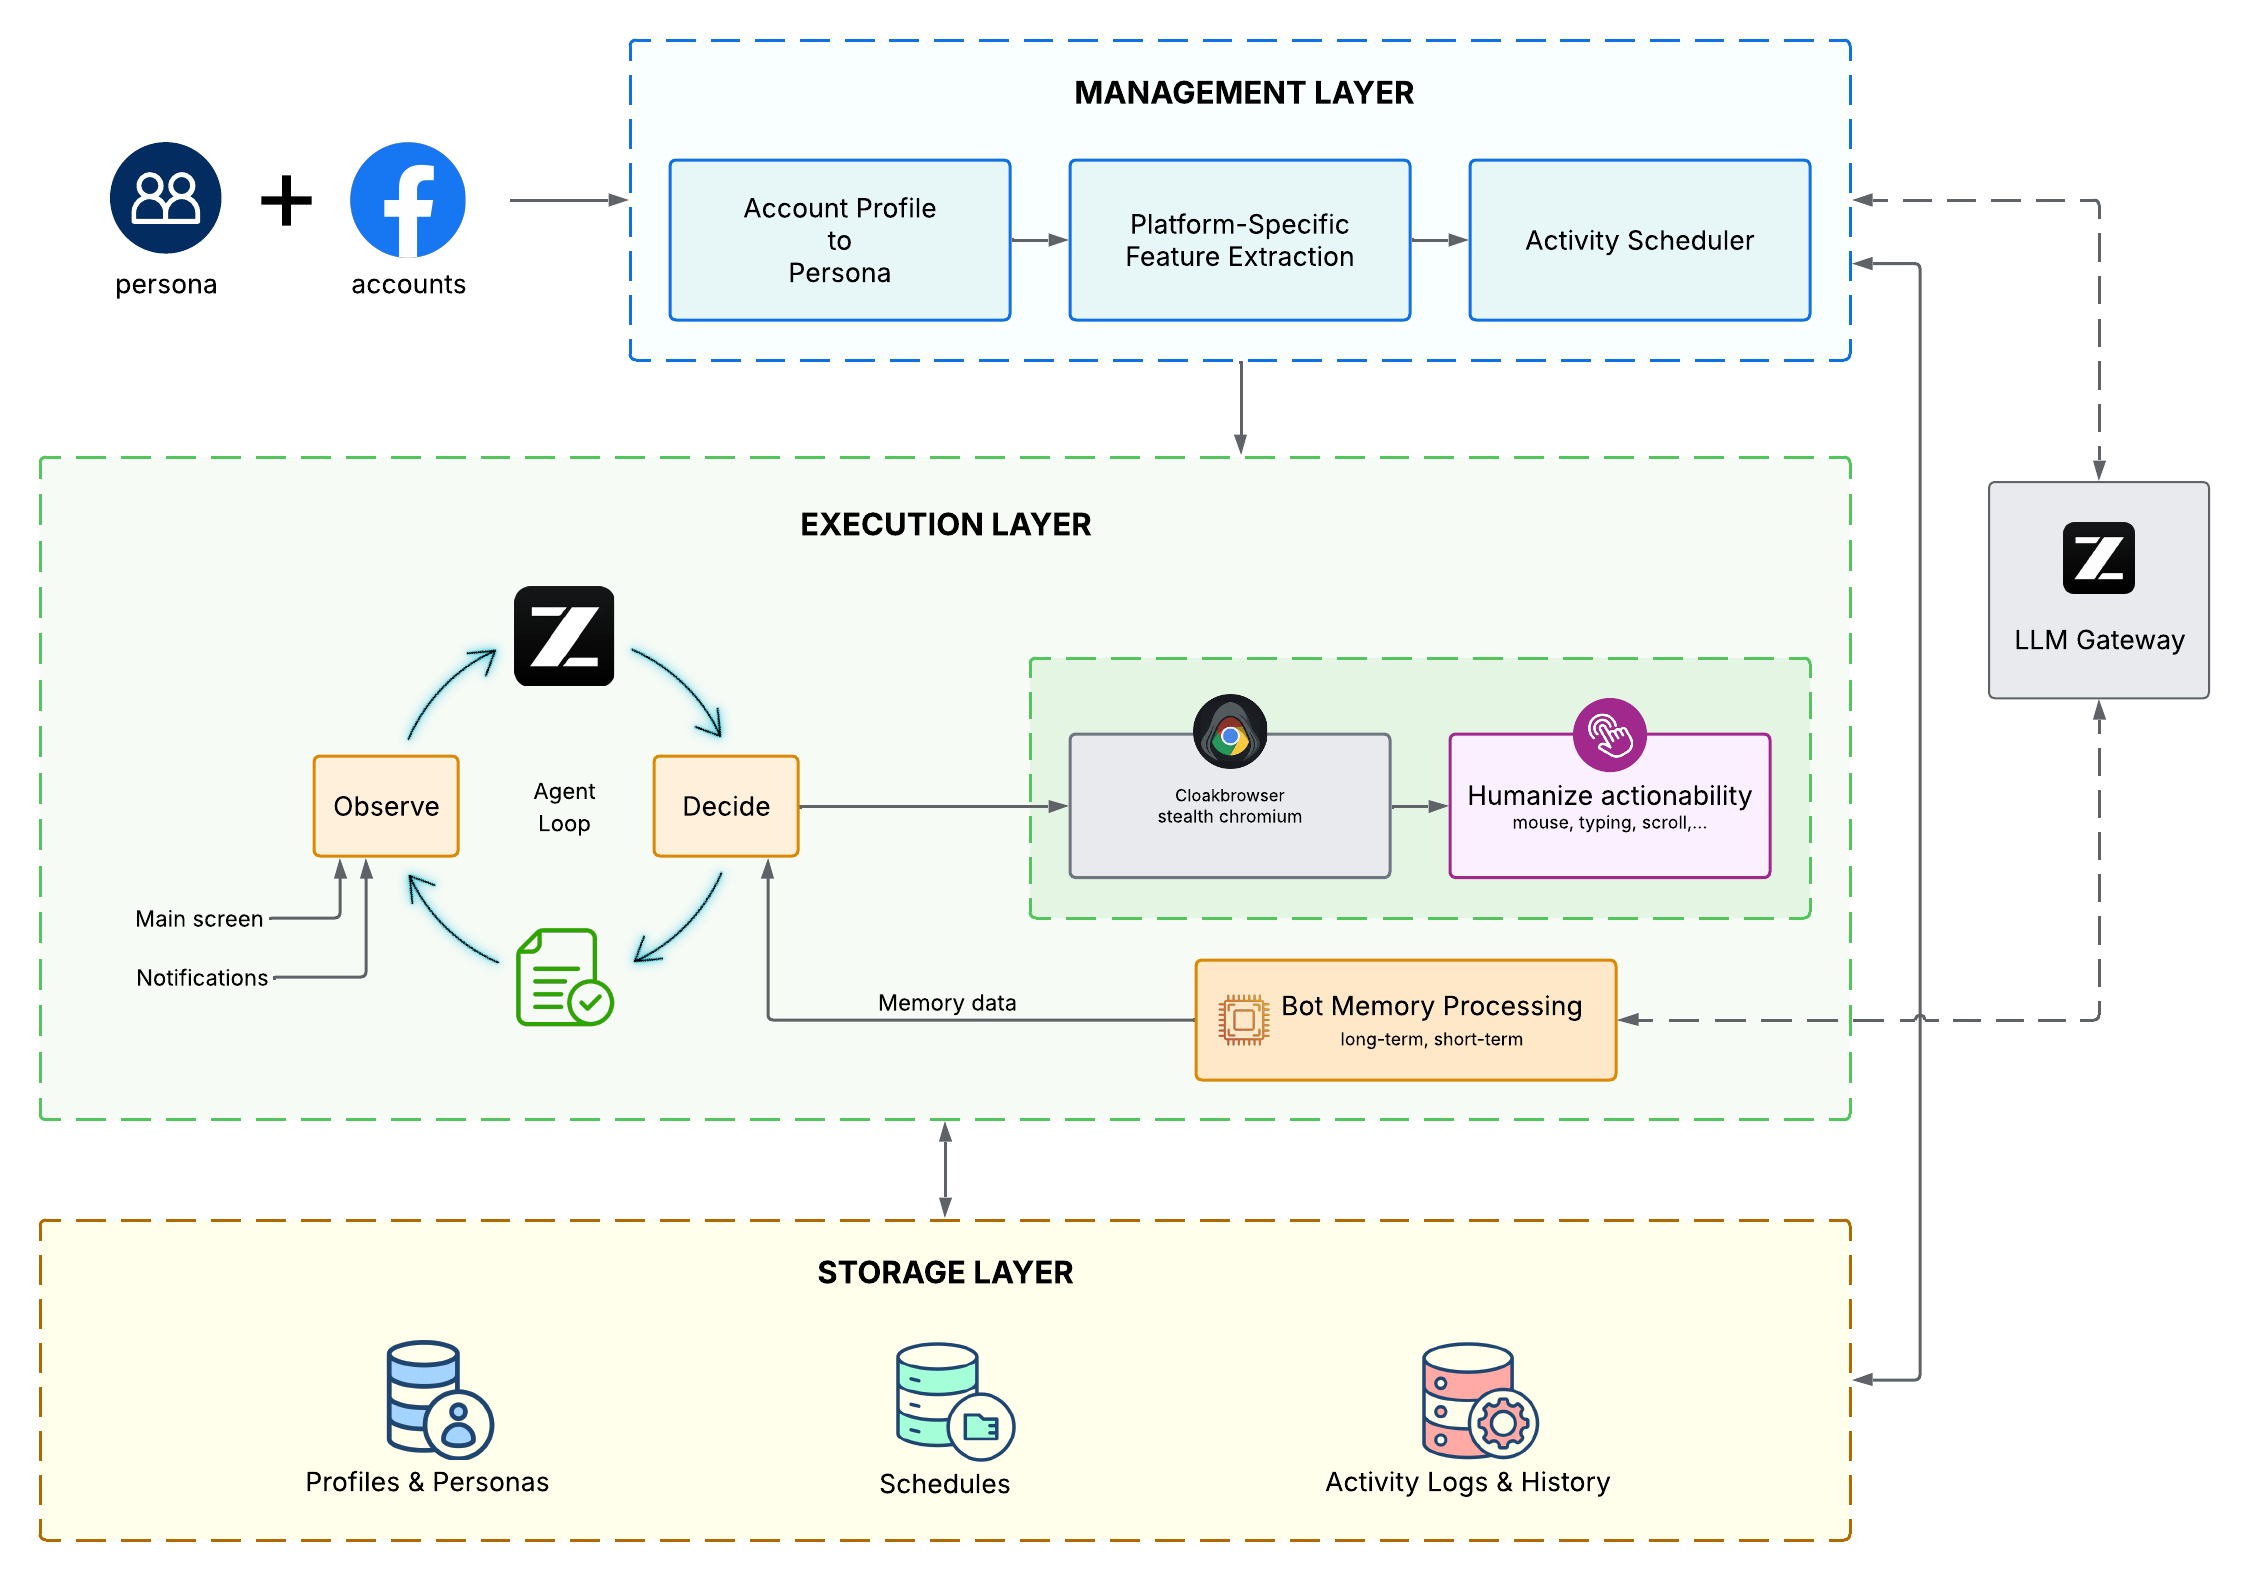
\includegraphics[keepaspectratio,alt={Kiến trúc Chu trình Vòng lặp Agent}]{../output/figures/agent_loop.png}}
\caption{Kiến trúc Chu trình Vòng lặp Agent}
\end{figure}

\subsubsection{Ba Tầng Hoạt động trong Chu trình Sinh Dữ
liệu:}\label{ba-tux1ea7ng-houx1ea1t-ux111ux1ed9ng-trong-chu-truxecnh-sinh-dux1eef-liux1ec7u}

\begin{enumerate}
\def\labelenumi{\arabic{enumi}.}
\tightlist
\item
  \textbf{Tầng Quản lý \& Khởi tạo Môi trường (Management Layer):}

  \begin{itemize}
  \tightlist
  \item
    \textbf{Đầu vào:} Ghép cặp hồ sơ người dùng (\texttt{Persona}) với
    tài khoản Facebook trắng hoàn toàn (\texttt{Fresh\ Accounts}) nhằm
    triệt tiêu thuật toán gợi ý của Meta.
  \item
    \textbf{Trích xuất \& Lập lịch:} Hệ thống chuẩn bị đặc trưng nền
    tảng Facebook (\texttt{Platform-Specific\ Feature\ Extraction}) và
    thiết lập ngân sách thời gian phiên chạy
    (\texttt{Activity\ Scheduler}).
  \end{itemize}
\item
  \textbf{Tầng Thực thi \& Vòng lặp Nhận thức - Hành động (Execution
  Layer - Agent Loop):} Vòng lặp diễn ra liên tục theo chu trình 4 pha
  tại mỗi bước tuần tự (\(S_t \rightarrow A_t\)):

  \begin{itemize}
  \tightlist
  \item
    \textbf{Observe (Quan sát):} Quét tín hiệu DOM từ màn hình chính
    (\texttt{Main\ screen}), bảng tin, bài viết trên viewport và thông
    báo (\texttt{Notifications}).
  \item
    \textbf{Decide (Ra quyết định):} Tác tử gửi ngữ cảnh qua
    \texttt{LLM\ Gateway} (DeepSeek Harness) kết hợp cùng
    \texttt{Bot\ Memory\ Processing} (bộ nhớ làm việc ngắn hạn
    \texttt{working\_memory} và ký ức phiên trước \texttt{long-term}) để
    lựa chọn ý định (\texttt{intent}), công cụ (\texttt{tool}), đối
    tượng mục tiêu (\texttt{target\_candidate}) và viện dẫn chiều tâm lý
    (\texttt{dimension\_evidence}).
  \item
    \textbf{Act \& Humanize (Thực thi cơ học):} Lệnh được chuyển qua
    trình duyệt ẩn danh \texttt{Cloakbrowser\ (stealth\ chromium)} và mô
    phỏng cử chỉ tự nhiên của con người
    (\texttt{Humanize\ actionability}: cuộn chuột mượt
    \texttt{smooth\_wheel}, ngắt nhịp thời gian \texttt{gesture\_ms},
    tốc độ \texttt{pace}, click ngẫu nhiên tọa độ).
  \item
    \textbf{Feedback \& State Update:} Nhận kết quả xác minh DOM
    (\texttt{verified}), cập nhật thời gian trôi qua, nạp lại bộ nhớ và
    quay lại pha \emph{Observe}.
  \end{itemize}
\item
  \textbf{Tầng Lưu trữ \& Cung cấp Dữ liệu EDA (Storage Layer):}

  \begin{itemize}
  \tightlist
  \item
    Mọi biến cố trong vòng lặp được ghi nhận tự động vào
    \textbf{\texttt{Activity\ Logs\ \&\ History}} để tiến hành EDA.
  \end{itemize}
\end{enumerate}

    \subsection{2.3. Cấu trúc Phân cấp 4 Tầng \& Đơn vị Phân tích
(Multi-level Data
Hierarchy)}\label{cux1ea5u-truxfac-phuxe2n-cux1ea5p-4-tux1ea7ng-ux111ux1a1n-vux1ecb-phuxe2n-tuxedch-multi-level-data-hierarchy}

\begin{verbatim}
Episode (N = 8) ---[1:N]---> Step (N = 437, Base Unit)
                               ├---[1:N]---> Browser Gesture (N = 189 actions, 63 gestures)
                               └---[1:N]---> Cognitive Evidence (N = 546 evidences)
\end{verbatim}

\subsubsection{Ma trận Đặc tính 4 Cấp độ Dữ
liệu:}\label{ma-trux1eadn-ux111ux1eb7c-tuxednh-4-cux1ea5p-ux111ux1ed9-dux1eef-liux1ec7u}

{\def\LTcaptype{none} % do not increment counter
\begin{longtable}[]{@{}
  >{\raggedright\arraybackslash}p{(\linewidth - 6\tabcolsep) * \real{0.2353}}
  >{\centering\arraybackslash}p{(\linewidth - 6\tabcolsep) * \real{0.2941}}
  >{\raggedright\arraybackslash}p{(\linewidth - 6\tabcolsep) * \real{0.2353}}
  >{\raggedright\arraybackslash}p{(\linewidth - 6\tabcolsep) * \real{0.2353}}@{}}
\toprule\noalign{}
\begin{minipage}[b]{\linewidth}\raggedright
Cấp độ
\end{minipage} & \begin{minipage}[b]{\linewidth}\centering
Quy mô (\(N\))
\end{minipage} & \begin{minipage}[b]{\linewidth}\raggedright
Ý nghĩa Phân tích
\end{minipage} & \begin{minipage}[b]{\linewidth}\raggedright
Đại lượng Đo lường Chính
\end{minipage} \\
\midrule\noalign{}
\endhead
\bottomrule\noalign{}
\endlastfoot
\textbf{1. Episode} & \textbf{8} phiên & Quan sát vĩ mô toàn phiên
(\textasciitilde10--12 phút) & Tổng thời lượng, tổng số bước, số bề mặt
ghé thăm, lý do dừng \\
\textbf{2. Step} & \textbf{437} bước & \textbf{Đơn vị phân tích cơ sở
(Base Unit)}: Quyết định \(S_t \rightarrow A_t\) & \texttt{intent},
\texttt{tool}, \texttt{surface}, \texttt{reaction}, \texttt{verified},
\texttt{latency\_ratio} \\
\textbf{3. Gesture} & \textbf{189} actions & Thao tác cơ học vật lý trên
trình duyệt & \texttt{gesture\_pace}, \texttt{gesture\_ms},
\texttt{gesture\_total\_px}, \texttt{execution\_mode} \\
\textbf{4. Evidence} & \textbf{546} items & Viện dẫn nhận thức \& chiều
tâm lý của Persona & \texttt{dimension}, \texttt{role}
(primary/secondary), \texttt{weight}, \texttt{ref\_id} \\
\end{longtable}
}

    \begin{tcolorbox}[breakable, size=fbox, boxrule=1pt, pad at break*=1mm,colback=cellbackground, colframe=cellborder]
\prompt{In}{incolor}{2}{\boxspacing}
\begin{Verbatim}[commandchars=\\\{\}]
\PY{c+c1}{\PYZsh{} Thực thi kiểm định cấu trúc phân cấp và kiểm tra toàn vẹn khóa ngoại (Referential Integrity)}
\PY{k+kn}{from}\PY{+w}{ }\PY{n+nn}{algorithms}\PY{n+nn}{.}\PY{n+nn}{data\PYZus{}lineage\PYZus{}inspector}\PY{+w}{ }\PY{k+kn}{import} \PY{n}{inspect\PYZus{}multilevel\PYZus{}structure}
\PY{k+kn}{from}\PY{+w}{ }\PY{n+nn}{viz}\PY{n+nn}{.}\PY{n+nn}{data\PYZus{}lineage\PYZus{}viz}\PY{+w}{ }\PY{k+kn}{import} \PY{n}{plot\PYZus{}data\PYZus{}hierarchy\PYZus{}distribution}

\PY{c+c1}{\PYZsh{} Nạp đầy đủ 4 cấp độ từ PersonaActionLoader}
\PY{n}{df\PYZus{}episodes} \PY{o}{=} \PY{n}{loader}\PY{o}{.}\PY{n}{load\PYZus{}action\PYZus{}logs}\PY{p}{(}\PY{p}{)}
\PY{n}{df\PYZus{}steps} \PY{o}{=} \PY{n}{loader}\PY{o}{.}\PY{n}{load\PYZus{}step\PYZus{}records}\PY{p}{(}\PY{p}{)}
\PY{n}{df\PYZus{}actions} \PY{o}{=} \PY{n}{loader}\PY{o}{.}\PY{n}{load\PYZus{}recent\PYZus{}actions}\PY{p}{(}\PY{p}{)}
\PY{n}{df\PYZus{}evidences} \PY{o}{=} \PY{n}{loader}\PY{o}{.}\PY{n}{load\PYZus{}dimension\PYZus{}evidences}\PY{p}{(}\PY{p}{)}

\PY{c+c1}{\PYZsh{} Kiểm tra toàn vẹn tham chiếu}
\PY{n}{lineage\PYZus{}audit} \PY{o}{=} \PY{n}{inspect\PYZus{}multilevel\PYZus{}structure}\PY{p}{(}\PY{n}{df\PYZus{}episodes}\PY{p}{,} \PY{n}{df\PYZus{}steps}\PY{p}{,} \PY{n}{df\PYZus{}actions}\PY{p}{,} \PY{n}{df\PYZus{}evidences}\PY{p}{)}
\PY{n}{df\PYZus{}hierarchy\PYZus{}summary} \PY{o}{=} \PY{n}{lineage\PYZus{}audit}\PY{p}{[}\PY{l+s+s2}{\PYZdq{}}\PY{l+s+s2}{summary\PYZus{}table}\PY{l+s+s2}{\PYZdq{}}\PY{p}{]}

\PY{c+c1}{\PYZsh{} Lưu bảng ra output/tables/}
\PY{n}{table\PYZus{}path} \PY{o}{=} \PY{n}{project\PYZus{}root} \PY{o}{/} \PY{l+s+s2}{\PYZdq{}}\PY{l+s+s2}{output}\PY{l+s+s2}{\PYZdq{}} \PY{o}{/} \PY{l+s+s2}{\PYZdq{}}\PY{l+s+s2}{tables}\PY{l+s+s2}{\PYZdq{}} \PY{o}{/} \PY{l+s+s2}{\PYZdq{}}\PY{l+s+s2}{step2\PYZus{}data\PYZus{}hierarchy.csv}\PY{l+s+s2}{\PYZdq{}}
\PY{n}{df\PYZus{}hierarchy\PYZus{}summary}\PY{o}{.}\PY{n}{to\PYZus{}csv}\PY{p}{(}\PY{n}{table\PYZus{}path}\PY{p}{,} \PY{n}{index}\PY{o}{=}\PY{k+kc}{False}\PY{p}{,} \PY{n}{encoding}\PY{o}{=}\PY{l+s+s2}{\PYZdq{}}\PY{l+s+s2}{utf\PYZhy{}8\PYZhy{}sig}\PY{l+s+s2}{\PYZdq{}}\PY{p}{)}

\PY{c+c1}{\PYZsh{} Vẽ biểu đồ phân bổ cấu trúc và lưu ra output/figures/}
\PY{n}{fig\PYZus{}path} \PY{o}{=} \PY{n}{project\PYZus{}root} \PY{o}{/} \PY{l+s+s2}{\PYZdq{}}\PY{l+s+s2}{output}\PY{l+s+s2}{\PYZdq{}} \PY{o}{/} \PY{l+s+s2}{\PYZdq{}}\PY{l+s+s2}{figures}\PY{l+s+s2}{\PYZdq{}} \PY{o}{/} \PY{l+s+s2}{\PYZdq{}}\PY{l+s+s2}{step2\PYZus{}data\PYZus{}hierarchy.png}\PY{l+s+s2}{\PYZdq{}}
\PY{n}{fig} \PY{o}{=} \PY{n}{plot\PYZus{}data\PYZus{}hierarchy\PYZus{}distribution}\PY{p}{(}\PY{n}{df\PYZus{}hierarchy\PYZus{}summary}\PY{p}{,} \PY{n}{fig\PYZus{}path}\PY{p}{)}
\PY{n}{plt}\PY{o}{.}\PY{n}{show}\PY{p}{(}\PY{p}{)}

\PY{n+nb}{print}\PY{p}{(}\PY{l+s+s2}{\PYZdq{}}\PY{l+s+s2}{[✓] BẢNG TỔNG HỢP CẤU TRÚC ĐA CẤP (UNITS OF ANALYSIS):}\PY{l+s+s2}{\PYZdq{}}\PY{p}{)}
\PY{n}{display}\PY{p}{(}\PY{n}{df\PYZus{}hierarchy\PYZus{}summary}\PY{p}{)}
\end{Verbatim}
\end{tcolorbox}

    \begin{Verbatim}[commandchars=\\\{\}]
[✓] Đã lưu biểu đồ cấu trúc dữ liệu tại:
D:\textbackslash{}source\_code\textbackslash{}eda\_persona\textbackslash{}output\textbackslash{}figures\textbackslash{}step2\_data\_hierarchy.png
    \end{Verbatim}

    \begin{center}
    \adjustimage{max size={0.9\linewidth}{0.9\paperheight}}{eda_action_logs_files/eda_action_logs_9_1.png}
    \end{center}
    { \hspace*{\fill} \\}
    
    \begin{Verbatim}[commandchars=\\\{\}]
[✓] BẢNG TỔNG HỢP CẤU TRÚC ĐA CẤP (UNITS OF ANALYSIS):
    \end{Verbatim}

    
    \begin{Verbatim}[commandchars=\\\{\}]
        Cấp độ phân tích (Unit of Analysis)  Tổng số bản ghi (N)  Nhóm Persona  Nhóm No-Persona                           Khóa chính (PK)                      Khóa ngoại (FK) Toàn vẹn tham chiếu
0                  1. Episode Level (Phiên)                    8             6                2                                episode\_id                                 None          100\% Valid
1                      2. Step Level (Bước)                  437           349               88                  (episode\_id, step\_index)             episode\_id -> Episode.PK          100\% Valid
2         3. Browser Gesture Level (Cử chỉ)                  189           168               21    (episode\_id, step\_index, action\_order)  (episode\_id, step\_index) -> Step.PK          100\% Valid
3  4. Cognitive Evidence Level (Bằng chứng)                  546           546                0  (episode\_id, step\_index, evidence\_order)  (episode\_id, step\_index) -> Step.PK          100\% Valid
    \end{Verbatim}

    
    \subsection{2.4. Data Dictionary (Từ điển Dữ liệu Toàn diện - 94 Trường
Cấp độ
Step)}\label{data-dictionary-tux1eeb-ux111iux1ec3n-dux1eef-liux1ec7u-touxe0n-diux1ec7n---94-trux1b0ux1eddng-cux1ea5p-ux111ux1ed9-step}

Trong \texttt{loaders/persona\_action.py}, dữ liệu từ log thô được bóc
tách và làm phẳng thành \textbf{94 trường phân tích} ở cấp độ bước
(\texttt{Step\ Level} --- đơn vị phân tích cơ sở). Toàn bộ 94 trường này
được tổ chức thành \textbf{11 nhóm chức năng logic}:

{\def\LTcaptype{none} % do not increment counter
\begin{longtable}[]{@{}
  >{\centering\arraybackslash}p{(\linewidth - 6\tabcolsep) * \real{0.2778}}
  >{\raggedright\arraybackslash}p{(\linewidth - 6\tabcolsep) * \real{0.2222}}
  >{\centering\arraybackslash}p{(\linewidth - 6\tabcolsep) * \real{0.2778}}
  >{\raggedright\arraybackslash}p{(\linewidth - 6\tabcolsep) * \real{0.2222}}@{}}
\toprule\noalign{}
\begin{minipage}[b]{\linewidth}\centering
STT
\end{minipage} & \begin{minipage}[b]{\linewidth}\raggedright
Nhóm Chức năng (Functional Group)
\end{minipage} & \begin{minipage}[b]{\linewidth}\centering
Số lượng Trường
\end{minipage} & \begin{minipage}[b]{\linewidth}\raggedright
Các biến tiêu biểu
\end{minipage} \\
\midrule\noalign{}
\endhead
\bottomrule\noalign{}
\endlastfoot
\textbf{1} & \textbf{Metadata \& Persona Attributes} & 8 &
\texttt{episode\_id}, \texttt{persona\_id}, \texttt{persona\_pace},
\texttt{persona\_rest\_style}, \texttt{dataset\_type},
\texttt{step\_index}, \texttt{timestamp} \\
\textbf{2} & \textbf{Action Space \& Execution Core} & 14 &
\texttt{tool}, \texttt{resolved\_tool}, \texttt{intent},
\texttt{reaction}, \texttt{surface}, \texttt{verified}, \texttt{reason},
\texttt{action\_summary\_verb} \\
\textbf{3} & \textbf{Latency \& Computational Effort} & 5 &
\texttt{model\_latency\_ms}, \texttt{tool\_execution\_ms},
\texttt{total\_step\_latency\_ms}, \texttt{cognitive\_latency\_ratio} \\
\textbf{4} & \textbf{Target Candidate (Content Selection)} & 4 &
\texttt{has\_target\_candidate}, \texttt{target\_candidate\_kind},
\texttt{target\_candidate\_text}, \texttt{target\_candidate\_url} \\
\textbf{5} & \textbf{Cognitive Reasoning Matrix} & 14 &
\texttt{dim\_evidence\_primary\_dimension},
\texttt{dim\_evidence\_max\_weight}, \texttt{num\_dim\_primary},
\texttt{num\_dim\_supporting} \\
\textbf{6} & \textbf{Session Context: Temporal Dynamics} & 6 &
\texttt{context\_elapsed\_seconds},
\texttt{context\_remaining\_seconds}, \texttt{context\_is\_overtime},
\texttt{context\_action\_velocity} \\
\textbf{7} & \textbf{Session Context: Rest \& Fatigue} & 2 &
\texttt{context\_rest\_accumulated\_seconds},
\texttt{context\_rest\_count} \\
\textbf{8} & \textbf{Session Context: Search \& Memory} & 7 &
\texttt{context\_queries\_this\_session},
\texttt{context\_recent\_queries\_from\_memory}, \texttt{search\_rule},
\texttt{planner\_rule} \\
\textbf{9} & \textbf{Session Context: Physical Gestures} & 12 &
\texttt{recent\_last\_gesture\_pace},
\texttt{recent\_last\_gesture\_px}, \texttt{recent\_last\_gesture\_ms},
\texttt{landing\_correction} \\
\textbf{10} & \textbf{Working Memory: Threads \& Anti-Drift} & 16 &
\texttt{wm\_current\_thread\_origin}, \texttt{wm\_situational\_steps},
\texttt{wm\_has\_novelty\_warning}, \texttt{wm\_novelty\_guidance} \\
\textbf{11} & \textbf{Working Memory: Session Summaries} & 6 &
\texttt{wm\_summary\_run\_minutes},
\texttt{wm\_summary\_planned\_minutes},
\texttt{wm\_summary\_read\_posts} \\
\textbf{TỔNG} & \textbf{Toàn bộ Không gian Biến số Cấp Step} &
\textbf{94} & \emph{Bao quát trọn vẹn chu trình Nhận thức
\(\rightarrow\) Quyết định \(\rightarrow\) Thực thi vật lý} \\
\end{longtable}
}

    \begin{tcolorbox}[breakable, size=fbox, boxrule=1pt, pad at break*=1mm,colback=cellbackground, colframe=cellborder]
\prompt{In}{incolor}{3}{\boxspacing}
\begin{Verbatim}[commandchars=\\\{\}]
\PY{c+c1}{\PYZsh{} Nạp và hiển thị Data Dictionary từ file chuẩn output/tables/data\PYZus{}dictionary.csv}
\PY{n}{dict\PYZus{}path} \PY{o}{=} \PY{n}{project\PYZus{}root} \PY{o}{/} \PY{l+s+s2}{\PYZdq{}}\PY{l+s+s2}{output}\PY{l+s+s2}{\PYZdq{}} \PY{o}{/} \PY{l+s+s2}{\PYZdq{}}\PY{l+s+s2}{tables}\PY{l+s+s2}{\PYZdq{}} \PY{o}{/} \PY{l+s+s2}{\PYZdq{}}\PY{l+s+s2}{data\PYZus{}dictionary.csv}\PY{l+s+s2}{\PYZdq{}}
\PY{n}{df\PYZus{}data\PYZus{}dict} \PY{o}{=} \PY{n}{pd}\PY{o}{.}\PY{n}{read\PYZus{}csv}\PY{p}{(}\PY{n}{dict\PYZus{}path}\PY{p}{)}

\PY{n+nb}{print}\PY{p}{(}\PY{l+s+sa}{f}\PY{l+s+s2}{\PYZdq{}}\PY{l+s+s2}{[✓] Tổng số trường then chốt trong Data Dictionary: }\PY{l+s+si}{\PYZob{}}\PY{n+nb}{len}\PY{p}{(}\PY{n}{df\PYZus{}data\PYZus{}dict}\PY{p}{)}\PY{l+s+si}{\PYZcb{}}\PY{l+s+s2}{ trường.}\PY{l+s+s2}{\PYZdq{}}\PY{p}{)}
\PY{n+nb}{print}\PY{p}{(}\PY{l+s+s2}{\PYZdq{}}\PY{l+s+s2}{[✓] Phân bổ theo 7 nhóm chính:}\PY{l+s+s2}{\PYZdq{}}\PY{p}{)}
\PY{n+nb}{print}\PY{p}{(}\PY{n}{df\PYZus{}data\PYZus{}dict}\PY{p}{[}\PY{l+s+s2}{\PYZdq{}}\PY{l+s+s2}{Group}\PY{l+s+s2}{\PYZdq{}}\PY{p}{]}\PY{o}{.}\PY{n}{value\PYZus{}counts}\PY{p}{(}\PY{p}{)}\PY{o}{.}\PY{n}{sort\PYZus{}index}\PY{p}{(}\PY{p}{)}\PY{p}{)}

\PY{c+c1}{\PYZsh{} Hiển thị toàn bộ từ điển dữ liệu với định dạng bảng chi tiết}
\PY{n}{df\PYZus{}data\PYZus{}dict}\PY{o}{.}\PY{n}{style}\PY{o}{.}\PY{n}{set\PYZus{}properties}\PY{p}{(}\PY{o}{*}\PY{o}{*}\PY{p}{\PYZob{}}
    \PY{l+s+s1}{\PYZsq{}}\PY{l+s+s1}{text\PYZhy{}align}\PY{l+s+s1}{\PYZsq{}}\PY{p}{:} \PY{l+s+s1}{\PYZsq{}}\PY{l+s+s1}{left}\PY{l+s+s1}{\PYZsq{}}\PY{p}{,}
    \PY{l+s+s1}{\PYZsq{}}\PY{l+s+s1}{white\PYZhy{}space}\PY{l+s+s1}{\PYZsq{}}\PY{p}{:} \PY{l+s+s1}{\PYZsq{}}\PY{l+s+s1}{pre\PYZhy{}wrap}\PY{l+s+s1}{\PYZsq{}}\PY{p}{,}
    \PY{l+s+s1}{\PYZsq{}}\PY{l+s+s1}{font\PYZhy{}size}\PY{l+s+s1}{\PYZsq{}}\PY{p}{:} \PY{l+s+s1}{\PYZsq{}}\PY{l+s+s1}{12px}\PY{l+s+s1}{\PYZsq{}}
\PY{p}{\PYZcb{}}\PY{p}{)}\PY{o}{.}\PY{n}{set\PYZus{}table\PYZus{}styles}\PY{p}{(}\PY{p}{[}
    \PY{n+nb}{dict}\PY{p}{(}\PY{n}{selector}\PY{o}{=}\PY{l+s+s1}{\PYZsq{}}\PY{l+s+s1}{th}\PY{l+s+s1}{\PYZsq{}}\PY{p}{,} \PY{n}{props}\PY{o}{=}\PY{p}{[}\PY{p}{(}\PY{l+s+s1}{\PYZsq{}}\PY{l+s+s1}{font\PYZhy{}weight}\PY{l+s+s1}{\PYZsq{}}\PY{p}{,} \PY{l+s+s1}{\PYZsq{}}\PY{l+s+s1}{bold}\PY{l+s+s1}{\PYZsq{}}\PY{p}{)}\PY{p}{,} \PY{p}{(}\PY{l+s+s1}{\PYZsq{}}\PY{l+s+s1}{background\PYZhy{}color}\PY{l+s+s1}{\PYZsq{}}\PY{p}{,} \PY{l+s+s1}{\PYZsq{}}\PY{l+s+s1}{\PYZsh{}f0f2f5}\PY{l+s+s1}{\PYZsq{}}\PY{p}{)}\PY{p}{,} \PY{p}{(}\PY{l+s+s1}{\PYZsq{}}\PY{l+s+s1}{text\PYZhy{}align}\PY{l+s+s1}{\PYZsq{}}\PY{p}{,} \PY{l+s+s1}{\PYZsq{}}\PY{l+s+s1}{center}\PY{l+s+s1}{\PYZsq{}}\PY{p}{)}\PY{p}{]}\PY{p}{)}
\PY{p}{]}\PY{p}{)}
\end{Verbatim}
\end{tcolorbox}

    \begin{Verbatim}[commandchars=\\\{\}]
[✓] Tổng số trường then chốt trong Data Dictionary: 94 trường.
[✓] Phân bổ theo 7 nhóm chính:
Group
1. Metadata \& Persona             8
10. Working Memory \& Drift       16
11. WM Session Summaries          6
2. Action Space \& Execution      14
3. Latency \& Effort               5
4. Target Candidate (Content)     4
5. Cognitive Matrix              14
6. Temporal Budget \& Dynamics     6
7. Rest \& Fatigue                 2
8. Search \& Memory                7
9. Browser Physical Gestures     12
Name: count, dtype: int64
    \end{Verbatim}

            \begin{tcolorbox}[breakable, size=fbox, boxrule=.5pt, pad at break*=1mm, opacityfill=0]
\prompt{Out}{outcolor}{3}{\boxspacing}
\begin{Verbatim}[commandchars=\\\{\}]
<pandas.io.formats.style.Styler at 0x1f61e490590>
\end{Verbatim}
\end{tcolorbox}
        
    \subsection{2.5. Ghi nhận Tiền Xử lý (Preprocessing) \& Kiểm soát Rủi ro
Thiên lệch (Bias
Audit)}\label{ghi-nhux1eadn-tiux1ec1n-xux1eed-luxfd-preprocessing-kiux1ec3m-souxe1t-rux1ee7i-ro-thiuxean-lux1ec7ch-bias-audit}

\subsubsection{\texorpdfstring{A. Các quy trình tiền xử lý đã thực hiện
trong
\texttt{PersonaActionLoader}:}{A. Các quy trình tiền xử lý đã thực hiện trong PersonaActionLoader:}}\label{a.-cuxe1c-quy-truxecnh-tiux1ec1n-xux1eed-luxfd-ux111uxe3-thux1ef1c-hiux1ec7n-trong-personaactionloader}

\begin{enumerate}
\def\labelenumi{\arabic{enumi}.}
\tightlist
\item
  \textbf{Bóc tách cấu trúc lồng nhau (Unnesting \& Flattening):}

  \begin{itemize}
  \tightlist
  \item
    Trích xuất \texttt{target\_candidate} (kind, text, url) từ cấu trúc
    dictionary lồng trong \texttt{step\_records}.
  \item
    Bóc tách mảng \texttt{dimension\_evidence} thành bảng quan hệ 1-N
    (546 bản ghi) và trích xuất chiều chính (\texttt{primary}) cùng
    trọng số cao nhất (\texttt{max\_weight}) lên cấp độ bước.
  \end{itemize}
\item
  \textbf{Trích xuất thuộc tính bằng Regular Expression:}

  \begin{itemize}
  \tightlist
  \item
    Sử dụng regex phân tích trường text
    \texttt{recent\_actions{[}{]}.summary} để thu nhận chính xác các
    tham số vật lý: \texttt{total=(\textbackslash{}d+)px},
    \texttt{gesture\_ms=(\textbackslash{}d+)},
    \texttt{pace=(fast\textbar{}careful)},
    \texttt{mode=(\textbackslash{}w+)}.
  \end{itemize}
\item
  \textbf{Chuẩn hóa biến thời gian \& ngân sách:}

  \begin{itemize}
  \tightlist
  \item
    Chuyển đổi timestamp ISO 8601 sang UTC datetime.
  \item
    Tính toán
    \texttt{cognitive\_latency\_ratio\ =\ model\_ms\ /\ (model\_ms\ +\ tool\_ms)}.
  \end{itemize}
\end{enumerate}

\subsubsection{B. Kiểm soát các Rủi ro Thiên lệch (Potential Biases \&
Mitigation):}\label{b.-kiux1ec3m-souxe1t-cuxe1c-rux1ee7i-ro-thiuxean-lux1ec7ch-potential-biases-mitigation}

{\def\LTcaptype{none} % do not increment counter
\begin{longtable}[]{@{}
  >{\raggedright\arraybackslash}p{(\linewidth - 6\tabcolsep) * \real{0.2500}}
  >{\raggedright\arraybackslash}p{(\linewidth - 6\tabcolsep) * \real{0.2500}}
  >{\raggedright\arraybackslash}p{(\linewidth - 6\tabcolsep) * \real{0.2500}}
  >{\raggedright\arraybackslash}p{(\linewidth - 6\tabcolsep) * \real{0.2500}}@{}}
\toprule\noalign{}
\begin{minipage}[b]{\linewidth}\raggedright
Tên Thiên lệch / Rủi ro
\end{minipage} & \begin{minipage}[b]{\linewidth}\raggedright
Nguồn gốc
\end{minipage} & \begin{minipage}[b]{\linewidth}\raggedright
Tác động tiềm ẩn
\end{minipage} & \begin{minipage}[b]{\linewidth}\raggedright
Biện pháp Kiểm soát \& Xử lý trong EDA
\end{minipage} \\
\midrule\noalign{}
\endhead
\bottomrule\noalign{}
\endlastfoot
\textbf{Cold-start Feed Bias} & Bảng tin Facebook mặc định của tài khoản
trắng & Facebook thường đẩy các video Reels trending hoặc tin tức giật
gân ngẫu nhiên lên đầu. Nhóm No-Persona có thể bị cuốn vào các bài này.
& Phân tích tách biệt tỷ lệ bài viết khớp Persona vs bài viết xu hướng
tự nhiên (\texttt{target\_candidate\_kind}). \\
\textbf{Mất cân bằng Cỡ mẫu (Sample Asymmetry)} & 6 phiên Persona
(\(N=349\)) vs 2 phiên No-Persona (\(N=88\)) & So sánh tổng số lượng
tuyệt đối sẽ bị sai lệch hoàn toàn. & \textbf{Luôn chuẩn hóa theo tỷ lệ
phần trăm (Proportions)}, tỷ lệ per-step, và áp dụng kiểm định phi tham
số (Mann-Whitney U, Bootstrap, Permutation tests). \\
\textbf{Khuyết thiếu Chọn lọc (Selective Missingness - MAR)} & Một số
trường chỉ tồn tại theo ngữ cảnh (ví dụ: \texttt{dim\_evidence} chỉ có ở
nhóm Persona; \texttt{gesture\_ms} chỉ có khi cuộn chuột). & Dễ bị nhầm
lẫn là dữ liệu bị mất (MCAR) và tự ý xóa bỏ dòng. & Xử lý khuyết thiếu
theo điều kiện nghiệp vụ: không xóa dòng, phân tích trên tập con hợp lệ
(ví dụ: chỉ đo tốc độ cuộn trên các bước cuộn chuột). \\
\textbf{Thiên lệch Thời lượng (Duration / Survival Bias)} & Các phiên
dừng vì các lý do khác nhau (\texttt{completed},
\texttt{overtime\_threshold\_exceeded}). & Bước cuối của phiên có thể có
hành vi vội vã hoặc kết thúc đột ngột. & Kiểm soát biến
\texttt{context\_is\_overtime} và phân tích riêng biệt các bước trong
thời hạn vs các bước quá giờ. \\
\end{longtable}
}

    \section{3: KIỂM TRA TỔNG QUAN VÀ CHẤT LƯỢNG DỮ
LIỆU}\label{kiux1ec3m-tra-tux1ed5ng-quan-vuxe0-chux1ea5t-lux1b0ux1ee3ng-dux1eef-liux1ec7u}

Mục tiêu của phần 3 là thực hiện kiểm tra toàn diện về độ tin cậy của
tập dữ liệu hành vi tác tử, bao gồm: kiểm tra trùng lặp, giá trị bất hợp
lệ, phân loại khuyết thiếu (MCAR/MAR/MNAR), giải thích điểm ngoại lai
(Outliers) và kiểm tra tính liên tục của chuỗi thời gian, xác định quyết
định xử lý dữ liệu.

\subsection{3.1. Đánh giá Tổng quan Dữ
liệu}\label{ux111uxe1nh-giuxe1-tux1ed5ng-quan-dux1eef-liux1ec7u}

\begin{itemize}
\tightlist
\item
  \textbf{Kích thước \& Dung lượng:} 437 dòng (bước hành động) và 94 cột
  phân tích.
\item
  \textbf{Tính toàn vẹn khóa:} Khóa chính
  \texttt{(episode\_id,\ step\_index)} không có bản ghi trùng lặp nào (0
  dòng duplicate PK).
\item
  \textbf{Giá trị bất hợp lệ:} 0 cột có số âm phi lý; không có timestamp
  tương lai; các chuỗi rỗng đã được chuẩn hóa.
\end{itemize}

    \begin{tcolorbox}[breakable, size=fbox, boxrule=1pt, pad at break*=1mm,colback=cellbackground, colframe=cellborder]
\prompt{In}{incolor}{4}{\boxspacing}
\begin{Verbatim}[commandchars=\\\{\}]
\PY{k+kn}{from}\PY{+w}{ }\PY{n+nn}{algorithms}\PY{n+nn}{.}\PY{n+nn}{data\PYZus{}quality\PYZus{}profiler}\PY{+w}{ }\PY{k+kn}{import} \PY{n}{profile\PYZus{}data\PYZus{}hygiene}

\PY{n}{hygiene\PYZus{}audit} \PY{o}{=} \PY{n}{profile\PYZus{}data\PYZus{}hygiene}\PY{p}{(}\PY{n}{df\PYZus{}steps}\PY{p}{,} \PY{n}{primary\PYZus{}key}\PY{o}{=}\PY{p}{[}\PY{l+s+s2}{\PYZdq{}}\PY{l+s+s2}{episode\PYZus{}id}\PY{l+s+s2}{\PYZdq{}}\PY{p}{,} \PY{l+s+s2}{\PYZdq{}}\PY{l+s+s2}{step\PYZus{}index}\PY{l+s+s2}{\PYZdq{}}\PY{p}{]}\PY{p}{)}
\PY{n}{df\PYZus{}hygiene\PYZus{}summary} \PY{o}{=} \PY{n}{hygiene\PYZus{}audit}\PY{p}{[}\PY{l+s+s2}{\PYZdq{}}\PY{l+s+s2}{summary\PYZus{}table}\PY{l+s+s2}{\PYZdq{}}\PY{p}{]}

\PY{c+c1}{\PYZsh{} Lưu bảng ra output/tables/}
\PY{n}{df\PYZus{}hygiene\PYZus{}summary}\PY{o}{.}\PY{n}{to\PYZus{}csv}\PY{p}{(}\PY{n}{project\PYZus{}root} \PY{o}{/} \PY{l+s+s2}{\PYZdq{}}\PY{l+s+s2}{output}\PY{l+s+s2}{\PYZdq{}} \PY{o}{/} \PY{l+s+s2}{\PYZdq{}}\PY{l+s+s2}{tables}\PY{l+s+s2}{\PYZdq{}} \PY{o}{/} \PY{l+s+s2}{\PYZdq{}}\PY{l+s+s2}{step3\PYZus{}quality\PYZus{}summary.csv}\PY{l+s+s2}{\PYZdq{}}\PY{p}{,} \PY{n}{index}\PY{o}{=}\PY{k+kc}{False}\PY{p}{,} \PY{n}{encoding}\PY{o}{=}\PY{l+s+s2}{\PYZdq{}}\PY{l+s+s2}{utf\PYZhy{}8\PYZhy{}sig}\PY{l+s+s2}{\PYZdq{}}\PY{p}{)}

\PY{n+nb}{print}\PY{p}{(}\PY{l+s+s2}{\PYZdq{}}\PY{l+s+s2}{[✓] BẢNG TỔNG HỢP KIỂM TRA VỆ SINH DỮ LIỆU:}\PY{l+s+s2}{\PYZdq{}}\PY{p}{)}
\PY{n}{display}\PY{p}{(}\PY{n}{df\PYZus{}hygiene\PYZus{}summary}\PY{p}{)}
\end{Verbatim}
\end{tcolorbox}

    \begin{Verbatim}[commandchars=\\\{\}]
[✓] BẢNG TỔNG HỢP KIỂM TRA VỆ SINH DỮ LIỆU:
    \end{Verbatim}

    
    \begin{Verbatim}[commandchars=\\\{\}]
                             Hạng mục kiểm tra  Kết quả thực tế     Tiêu chuẩn kỳ vọng     Trạng thái
0                        Tổng số dòng (N\_rows)         437 dòng             > 400 dòng            Đạt
1                         Tổng số cột (N\_cols)           94 cột              >= 90 cột            Đạt
2                        Dung lượng bộ nhớ RAM          2.12 MB                < 50 MB         Tối ưu
3  Trùng lặp dòng hoàn toàn (Exact Duplicates)           0 dòng                 0 dòng            Đạt
4         Trùng lặp khóa chính (PK Duplicates)           0 dòng                 0 dòng            Đạt
5       Giá trị âm phi logic (Negative values)    0 cột vi phạm                  0 cột            Đạt
6          Timestamp tương lai / Lỗi thời gian        0 bản ghi              0 bản ghi            Đạt
7    Chuỗi rỗng placeholder ẩn ('', N/A, null)  2 cột phát hiện  Đã bóc tách thành NaN  Cần chuẩn hóa
    \end{Verbatim}

    
    \subsection{3.2. Phân tích Cơ chế Khuyết
thiếu.}\label{phuxe2n-tuxedch-cux1a1-chux1ebf-khuyux1ebft-thiux1ebfu.}

\begin{quote}
\textbf{CƠ CHẾ `MISSING BY DESIGN' (KHUYẾT THIẾU CÓ ĐIỀU KIỆN NGHIỆP
VỤ):} Không thể tùy tiện áp dụng các kỹ thuật imputation (điền trung
bình/kNN) hoặc xóa bỏ dòng (listwise deletion) cho các giá trị NaN trong
tập dữ liệu này. Phần lớn dữ liệu thiếu tuân theo cơ chế \textbf{MAR
(Missing at Random)} bắt nguồn từ thiết kế thực nghiệm: - \textbf{Nhóm
trường \texttt{dim\_evidence\_*} (Bằng chứng nhận thức):} Khuyết 100\% ở
nhóm No-Persona (88 bước) vì nhóm đối chứng không có hồ sơ Persona để mô
hình viện dẫn. Ở nhóm Persona, trường này chỉ xuất hiện khi bước đó có
lý lẽ tâm lý. - \textbf{Nhóm trường \texttt{recent\_last\_gesture\_*}
(Cơ học cuộn):} Chỉ xuất hiện khi Agent thực hiện thao tác cuộn chuột
(\texttt{smooth\_wheel}), hoàn toàn không xuất hiện ở bước quan sát hay
click. - \textbf{Nhóm trường \texttt{target\_candidate\_*} (Thực thể bài
viết):} Chỉ xuất hiện ở 66 bước Agent chọn tương tác trúng một thực thể
cụ thể, các bước lướt bảng tin chung là NaN tự nhiên. - \textbf{Trường
\texttt{wm\_current\_thread\_state}:} Được bóc tách chính xác bằng cách
tra cứu trạng thái mạch từ \texttt{active\_threads} theo \texttt{topic},
thu được 343 bước có giá trị (333 `exploring', 10 `active') ở nhóm
Persona và khuyết 100\% ở nhóm đối chứng -\textgreater{} Thuộc cơ chế
MAR hoàn hảo (Memory-Thread Dependent).
\end{quote}

    \begin{tcolorbox}[breakable, size=fbox, boxrule=1pt, pad at break*=1mm,colback=cellbackground, colframe=cellborder]
\prompt{In}{incolor}{5}{\boxspacing}
\begin{Verbatim}[commandchars=\\\{\}]
\PY{k+kn}{from}\PY{+w}{ }\PY{n+nn}{algorithms}\PY{n+nn}{.}\PY{n+nn}{missing\PYZus{}pattern\PYZus{}analyzer}\PY{+w}{ }\PY{k+kn}{import} \PY{n}{analyze\PYZus{}missing\PYZus{}patterns}
\PY{k+kn}{from}\PY{+w}{ }\PY{n+nn}{viz}\PY{n+nn}{.}\PY{n+nn}{data\PYZus{}quality\PYZus{}viz}\PY{+w}{ }\PY{k+kn}{import} \PY{n}{plot\PYZus{}missing\PYZus{}patterns\PYZus{}comparison}

\PY{n}{missing\PYZus{}audit} \PY{o}{=} \PY{n}{analyze\PYZus{}missing\PYZus{}patterns}\PY{p}{(}\PY{n}{df\PYZus{}steps}\PY{p}{)}
\PY{n}{df\PYZus{}missing\PYZus{}report} \PY{o}{=} \PY{n}{missing\PYZus{}audit}\PY{p}{[}\PY{l+s+s2}{\PYZdq{}}\PY{l+s+s2}{missing\PYZus{}table}\PY{l+s+s2}{\PYZdq{}}\PY{p}{]}

\PY{c+c1}{\PYZsh{} Lưu bảng chi tiết}
\PY{n}{df\PYZus{}missing\PYZus{}report}\PY{o}{.}\PY{n}{to\PYZus{}csv}\PY{p}{(}\PY{n}{project\PYZus{}root} \PY{o}{/} \PY{l+s+s2}{\PYZdq{}}\PY{l+s+s2}{output}\PY{l+s+s2}{\PYZdq{}} \PY{o}{/} \PY{l+s+s2}{\PYZdq{}}\PY{l+s+s2}{tables}\PY{l+s+s2}{\PYZdq{}} \PY{o}{/} \PY{l+s+s2}{\PYZdq{}}\PY{l+s+s2}{step3\PYZus{}missing\PYZus{}analysis.csv}\PY{l+s+s2}{\PYZdq{}}\PY{p}{,} \PY{n}{index}\PY{o}{=}\PY{k+kc}{False}\PY{p}{,} \PY{n}{encoding}\PY{o}{=}\PY{l+s+s2}{\PYZdq{}}\PY{l+s+s2}{utf\PYZhy{}8\PYZhy{}sig}\PY{l+s+s2}{\PYZdq{}}\PY{p}{)}

\PY{c+c1}{\PYZsh{} Vẽ biểu đồ đối sánh tỷ lệ khuyết thiếu Top 15 biến}
\PY{n}{fig\PYZus{}missing} \PY{o}{=} \PY{n}{plot\PYZus{}missing\PYZus{}patterns\PYZus{}comparison}\PY{p}{(}
    \PY{n}{df\PYZus{}missing\PYZus{}report}\PY{p}{,}
    \PY{n}{output\PYZus{}path}\PY{o}{=}\PY{n}{project\PYZus{}root} \PY{o}{/} \PY{l+s+s2}{\PYZdq{}}\PY{l+s+s2}{output}\PY{l+s+s2}{\PYZdq{}} \PY{o}{/} \PY{l+s+s2}{\PYZdq{}}\PY{l+s+s2}{figures}\PY{l+s+s2}{\PYZdq{}} \PY{o}{/} \PY{l+s+s2}{\PYZdq{}}\PY{l+s+s2}{step3\PYZus{}missing\PYZus{}pattern.png}\PY{l+s+s2}{\PYZdq{}}\PY{p}{,}
    \PY{n}{top\PYZus{}n}\PY{o}{=}\PY{l+m+mi}{15}
\PY{p}{)}
\PY{n}{plt}\PY{o}{.}\PY{n}{show}\PY{p}{(}\PY{p}{)}

\PY{n+nb}{print}\PY{p}{(}\PY{l+s+s2}{\PYZdq{}}\PY{l+s+s2}{[✓] TOP 10 BIẾN CÓ TỶ LỆ KHUYẾT THIẾU CAO NHẤT \PYZam{} CƠ CHẾ NGHIỆP VỤ:}\PY{l+s+s2}{\PYZdq{}}\PY{p}{)}
\PY{n}{display}\PY{p}{(}\PY{n}{df\PYZus{}missing\PYZus{}report}\PY{o}{.}\PY{n}{head}\PY{p}{(}\PY{l+m+mi}{10}\PY{p}{)}\PY{p}{[}\PY{p}{[}\PY{l+s+s2}{\PYZdq{}}\PY{l+s+s2}{Field}\PY{l+s+s2}{\PYZdq{}}\PY{p}{,} \PY{l+s+s2}{\PYZdq{}}\PY{l+s+s2}{Missing\PYZus{}Pct}\PY{l+s+s2}{\PYZdq{}}\PY{p}{,} \PY{l+s+s2}{\PYZdq{}}\PY{l+s+s2}{Persona\PYZus{}Missing\PYZus{}Pct}\PY{l+s+s2}{\PYZdq{}}\PY{p}{,} \PY{l+s+s2}{\PYZdq{}}\PY{l+s+s2}{NoPersona\PYZus{}Missing\PYZus{}Pct}\PY{l+s+s2}{\PYZdq{}}\PY{p}{,} \PY{l+s+s2}{\PYZdq{}}\PY{l+s+s2}{Missing\PYZus{}Mechanism}\PY{l+s+s2}{\PYZdq{}}\PY{p}{,} \PY{l+s+s2}{\PYZdq{}}\PY{l+s+s2}{Business\PYZus{}Explanation}\PY{l+s+s2}{\PYZdq{}}\PY{p}{]}\PY{p}{]}\PY{p}{)}
\end{Verbatim}
\end{tcolorbox}

    \begin{Verbatim}[commandchars=\\\{\}]
[✓] Đã lưu biểu đồ missing pattern tại:
D:\textbackslash{}source\_code\textbackslash{}eda\_persona\textbackslash{}output\textbackslash{}figures\textbackslash{}step3\_missing\_pattern.png
    \end{Verbatim}

    \begin{center}
    \adjustimage{max size={0.9\linewidth}{0.9\paperheight}}{eda_action_logs_files/eda_action_logs_16_1.png}
    \end{center}
    { \hspace*{\fill} \\}
    
    \begin{Verbatim}[commandchars=\\\{\}]
[✓] TOP 10 BIẾN CÓ TỶ LỆ KHUYẾT THIẾU CAO NHẤT \& CƠ CHẾ NGHIỆP VỤ:
    \end{Verbatim}

    
    \begin{Verbatim}[commandchars=\\\{\}]
                                Field  Missing\_Pct  Persona\_Missing\_Pct  NoPersona\_Missing\_Pct          Missing\_Mechanism                               Business\_Explanation
0  context\_recent\_queries\_from\_memory       93.590               91.980                100.000   MAR (Memory-Conditional)  Chỉ xuất hiện ở 28 bước có nạp lại từ khóa từ {\ldots}
1         dim\_evidence\_primary\_ref\_id       88.790               87.390                 94.320    MAR (Missing by Design)  Khuyết 100\% ở nhóm No-Persona (do không có hồ {\ldots}
2          dim\_evidence\_reference\_ids       88.790               87.390                 94.320    MAR (Missing by Design)  Khuyết 100\% ở nhóm No-Persona (do không có hồ {\ldots}
3                target\_candidate\_url       84.900               82.810                 93.180  MAR (Content-Conditional)  Chỉ xuất hiện khi bước hành vi nhắm trúng thực{\ldots}
4               target\_candidate\_kind       84.900               82.810                 93.180  MAR (Content-Conditional)  Chỉ xuất hiện khi bước hành vi nhắm trúng thực{\ldots}
5               target\_candidate\_text       84.900               82.810                 93.180  MAR (Content-Conditional)  Chỉ xuất hiện khi bước hành vi nhắm trúng thực{\ldots}
6      recent\_last\_landing\_correction       81.920               77.940                 97.730      MAR (Group Dependent)  Tỷ lệ khuyết thiếu có sự phân hóa đáng kể giữa{\ldots}
7              recent\_last\_gesture\_ms       74.600               70.200                 92.050   MAR (Action-Conditional)  Chỉ xuất hiện ở bước có thao tác cuộn chuột (s{\ldots}
8            recent\_last\_gesture\_pace       74.600               70.200                 92.050   MAR (Action-Conditional)  Chỉ xuất hiện ở bước có thao tác cuộn chuột (s{\ldots}
9              recent\_last\_gesture\_px       74.600               70.200                 92.050   MAR (Action-Conditional)  Chỉ xuất hiện ở bước có thao tác cuộn chuột (s{\ldots}
    \end{Verbatim}

    
    \subsection{3.3. Thẩm định Điểm Dị biệt (Outliers): Lỗi Kỹ thuật hay Tín
hiệu
Thật?}\label{thux1ea9m-ux111ux1ecbnh-ux111iux1ec3m-dux1ecb-biux1ec7t-outliers-lux1ed7i-kux1ef9-thuux1eadt-hay-tuxedn-hiux1ec7u-thux1eadt}

Áp dụng phương pháp Hàng rào IQR của Tukey
(\(Q_1 - 1.5\times\text{IQR}\) và \(Q_3 + 1.5\times\text{IQR}\)): -
\textbf{\texttt{recent\_last\_gesture\_px} (7 outliers, 6.31\%):} Xuất
hiện các bước cuộn chuột dài đột biến (\textgreater{} 1,000 px, tối đa
1,418 px). Đây là \textbf{Tín hiệu Hành vi Thật (True Behavioral
Signal)} phản ánh chính xác phong cách lướt nhanh
(\texttt{readingDepth\ =\ skim} và \texttt{pace\ =\ quick}) của Persona
Huỳnh Tuấn Kiệt hoặc Lê Hoàng Long. \textbf{Quyết định: Giữ nguyên tuyệt
đối!} - \textbf{\texttt{wm\_situational\_steps} (56 outliers, 12.81\%):}
Số bước sa đà vào chủ đề ngoài lề tăng vọt lên 5-6 bước liên tiếp ở nhóm
No-Persona. Đây là \textbf{Bằng chứng Nghiên cứu Cốt lõi} về hiện tượng
Trôi dạt Nhận thức (Cognitive Drift) khi không có Persona điều hướng.
\textbf{Quyết định: Giữ nguyên!} - \textbf{\texttt{model\_latency\_ms}
\& \texttt{tool\_execution\_ms}:} Biến thiên độ trễ do mạng và kích
thước trang Facebook. Áp dụng các kiểm định phi tham số (Non-parametric
tests: Mann-Whitney U) để không bị ảnh hưởng bởi đuôi phân phối dài.

    \begin{tcolorbox}[breakable, size=fbox, boxrule=1pt, pad at break*=1mm,colback=cellbackground, colframe=cellborder]
\prompt{In}{incolor}{6}{\boxspacing}
\begin{Verbatim}[commandchars=\\\{\}]
\PY{c+c1}{\PYZsh{} 3.3. Phát hiện Outlier và trực quan hóa phân bố đối sánh}
\PY{k+kn}{from}\PY{+w}{ }\PY{n+nn}{algorithms}\PY{n+nn}{.}\PY{n+nn}{outlier\PYZus{}detector}\PY{+w}{ }\PY{k+kn}{import} \PY{n}{detect\PYZus{}outliers\PYZus{}iqr\PYZus{}mad}
\PY{k+kn}{from}\PY{+w}{ }\PY{n+nn}{viz}\PY{n+nn}{.}\PY{n+nn}{data\PYZus{}quality\PYZus{}viz}\PY{+w}{ }\PY{k+kn}{import} \PY{n}{plot\PYZus{}outliers\PYZus{}boxplots}

\PY{n}{outlier\PYZus{}audit} \PY{o}{=} \PY{n}{detect\PYZus{}outliers\PYZus{}iqr\PYZus{}mad}\PY{p}{(}\PY{n}{df\PYZus{}steps}\PY{p}{)}
\PY{n}{df\PYZus{}outliers\PYZus{}report} \PY{o}{=} \PY{n}{outlier\PYZus{}audit}\PY{p}{[}\PY{l+s+s2}{\PYZdq{}}\PY{l+s+s2}{outlier\PYZus{}table}\PY{l+s+s2}{\PYZdq{}}\PY{p}{]}

\PY{c+c1}{\PYZsh{} Lưu bảng}
\PY{n}{df\PYZus{}outliers\PYZus{}report}\PY{o}{.}\PY{n}{to\PYZus{}csv}\PY{p}{(}\PY{n}{project\PYZus{}root} \PY{o}{/} \PY{l+s+s2}{\PYZdq{}}\PY{l+s+s2}{output}\PY{l+s+s2}{\PYZdq{}} \PY{o}{/} \PY{l+s+s2}{\PYZdq{}}\PY{l+s+s2}{tables}\PY{l+s+s2}{\PYZdq{}} \PY{o}{/} \PY{l+s+s2}{\PYZdq{}}\PY{l+s+s2}{step3\PYZus{}outliers.csv}\PY{l+s+s2}{\PYZdq{}}\PY{p}{,} \PY{n}{index}\PY{o}{=}\PY{k+kc}{False}\PY{p}{,} \PY{n}{encoding}\PY{o}{=}\PY{l+s+s2}{\PYZdq{}}\PY{l+s+s2}{utf\PYZhy{}8\PYZhy{}sig}\PY{l+s+s2}{\PYZdq{}}\PY{p}{)}

\PY{c+c1}{\PYZsh{} Vẽ boxplots đối sánh 4 biến số cốt lõi}
\PY{n}{fig\PYZus{}outliers} \PY{o}{=} \PY{n}{plot\PYZus{}outliers\PYZus{}boxplots}\PY{p}{(}
    \PY{n}{df\PYZus{}steps}\PY{p}{,}
    \PY{n}{output\PYZus{}path}\PY{o}{=}\PY{n}{project\PYZus{}root} \PY{o}{/} \PY{l+s+s2}{\PYZdq{}}\PY{l+s+s2}{output}\PY{l+s+s2}{\PYZdq{}} \PY{o}{/} \PY{l+s+s2}{\PYZdq{}}\PY{l+s+s2}{figures}\PY{l+s+s2}{\PYZdq{}} \PY{o}{/} \PY{l+s+s2}{\PYZdq{}}\PY{l+s+s2}{step3\PYZus{}outlier\PYZus{}distribution.png}\PY{l+s+s2}{\PYZdq{}}
\PY{p}{)}
\PY{n}{plt}\PY{o}{.}\PY{n}{show}\PY{p}{(}\PY{p}{)}

\PY{n+nb}{print}\PY{p}{(}\PY{l+s+s2}{\PYZdq{}}\PY{l+s+s2}{[✓] BẢNG TỔNG HỢP NGOẠI LAI VÀ THẨM ĐỊNH BẢN CHẤT:}\PY{l+s+s2}{\PYZdq{}}\PY{p}{)}
\PY{n}{display}\PY{p}{(}\PY{n}{df\PYZus{}outliers\PYZus{}report}\PY{p}{[}\PY{p}{[}\PY{l+s+s2}{\PYZdq{}}\PY{l+s+s2}{Biến số}\PY{l+s+s2}{\PYZdq{}}\PY{p}{,} \PY{l+s+s2}{\PYZdq{}}\PY{l+s+s2}{Cỡ mẫu hợp lệ (N)}\PY{l+s+s2}{\PYZdq{}}\PY{p}{,} \PY{l+s+s2}{\PYZdq{}}\PY{l+s+s2}{Trung vị (Median)}\PY{l+s+s2}{\PYZdq{}}\PY{p}{,} \PY{l+s+s2}{\PYZdq{}}\PY{l+s+s2}{Số Outlier}\PY{l+s+s2}{\PYZdq{}}\PY{p}{,} \PY{l+s+s2}{\PYZdq{}}\PY{l+s+s2}{Tỷ lệ Outlier (}\PY{l+s+s2}{\PYZpc{}}\PY{l+s+s2}{)}\PY{l+s+s2}{\PYZdq{}}\PY{p}{,} \PY{l+s+s2}{\PYZdq{}}\PY{l+s+s2}{Bản chất Ngoại lai}\PY{l+s+s2}{\PYZdq{}}\PY{p}{,} \PY{l+s+s2}{\PYZdq{}}\PY{l+s+s2}{Quyết định Xử lý}\PY{l+s+s2}{\PYZdq{}}\PY{p}{]}\PY{p}{]}\PY{p}{)}
\end{Verbatim}
\end{tcolorbox}

    \begin{Verbatim}[commandchars=\\\{\}]
D:\textbackslash{}source\_code\textbackslash{}eda\_persona\textbackslash{}viz\textbackslash{}data\_quality\_viz.py:96: FutureWarning:

Passing `palette` without assigning `hue` is deprecated and will be removed in
v0.14.0. Assign the `x` variable to `hue` and set `legend=False` for the same
effect.

  sns.boxplot(
D:\textbackslash{}source\_code\textbackslash{}eda\_persona\textbackslash{}viz\textbackslash{}data\_quality\_viz.py:119: UserWarning:
set\_ticklabels() should only be used with a fixed number of ticks, i.e. after
set\_ticks() or using a FixedLocator. Otherwise, ticks may be mislabeled.
  ax.set\_xticklabels(["Persona (Can thiệp)", "No-Persona (Đối chứng)"])
D:\textbackslash{}source\_code\textbackslash{}eda\_persona\textbackslash{}viz\textbackslash{}data\_quality\_viz.py:96: FutureWarning:

Passing `palette` without assigning `hue` is deprecated and will be removed in
v0.14.0. Assign the `x` variable to `hue` and set `legend=False` for the same
effect.

  sns.boxplot(
D:\textbackslash{}source\_code\textbackslash{}eda\_persona\textbackslash{}viz\textbackslash{}data\_quality\_viz.py:119: UserWarning:
set\_ticklabels() should only be used with a fixed number of ticks, i.e. after
set\_ticks() or using a FixedLocator. Otherwise, ticks may be mislabeled.
  ax.set\_xticklabels(["Persona (Can thiệp)", "No-Persona (Đối chứng)"])
D:\textbackslash{}source\_code\textbackslash{}eda\_persona\textbackslash{}viz\textbackslash{}data\_quality\_viz.py:96: FutureWarning:

Passing `palette` without assigning `hue` is deprecated and will be removed in
v0.14.0. Assign the `x` variable to `hue` and set `legend=False` for the same
effect.

  sns.boxplot(
D:\textbackslash{}source\_code\textbackslash{}eda\_persona\textbackslash{}viz\textbackslash{}data\_quality\_viz.py:119: UserWarning:
set\_ticklabels() should only be used with a fixed number of ticks, i.e. after
set\_ticks() or using a FixedLocator. Otherwise, ticks may be mislabeled.
  ax.set\_xticklabels(["Persona (Can thiệp)", "No-Persona (Đối chứng)"])
D:\textbackslash{}source\_code\textbackslash{}eda\_persona\textbackslash{}viz\textbackslash{}data\_quality\_viz.py:96: FutureWarning:

Passing `palette` without assigning `hue` is deprecated and will be removed in
v0.14.0. Assign the `x` variable to `hue` and set `legend=False` for the same
effect.

  sns.boxplot(
D:\textbackslash{}source\_code\textbackslash{}eda\_persona\textbackslash{}viz\textbackslash{}data\_quality\_viz.py:119: UserWarning:
set\_ticklabels() should only be used with a fixed number of ticks, i.e. after
set\_ticks() or using a FixedLocator. Otherwise, ticks may be mislabeled.
  ax.set\_xticklabels(["Persona (Can thiệp)", "No-Persona (Đối chứng)"])
    \end{Verbatim}

    \begin{Verbatim}[commandchars=\\\{\}]
[✓] Đã lưu biểu đồ outlier distribution tại:
D:\textbackslash{}source\_code\textbackslash{}eda\_persona\textbackslash{}output\textbackslash{}figures\textbackslash{}step3\_outlier\_distribution.png
    \end{Verbatim}

    \begin{center}
    \adjustimage{max size={0.9\linewidth}{0.9\paperheight}}{eda_action_logs_files/eda_action_logs_18_2.png}
    \end{center}
    { \hspace*{\fill} \\}
    
    \begin{Verbatim}[commandchars=\\\{\}]
[✓] BẢNG TỔNG HỢP NGOẠI LAI VÀ THẨM ĐỊNH BẢN CHẤT:
    \end{Verbatim}

    
    \begin{Verbatim}[commandchars=\\\{\}]
                   Biến số  Cỡ mẫu hợp lệ (N)  Trung vị (Median)  Số Outlier  Tỷ lệ Outlier (\%)                                 Bản chất Ngoại lai                                   Quyết định Xử lý
0     wm\_situational\_steps                437              0.000          56             12.810     Tín hiệu Hành vi Thật (True Behavioral Signal)    GIỮ NGUYÊN (Không xóa bỏ, đưa vào phân tích RQ)
1        tool\_execution\_ms                437           4872.000          53             12.130  Biến thiên Hệ thống \& Độ trễ Mạng (System Late{\ldots}  GIỮ NGUYÊN (Sử dụng trung vị và kiểm định phi {\ldots}
2    total\_step\_latency\_ms                437           8343.000          51             11.670  Biến thiên Hệ thống \& Độ trễ Mạng (System Late{\ldots}  GIỮ NGUYÊN (Sử dụng trung vị và kiểm định phi {\ldots}
3   recent\_last\_gesture\_px                111            492.000           7              6.310     Tín hiệu Hành vi Thật (True Behavioral Signal)    GIỮ NGUYÊN (Không xóa bỏ, đưa vào phân tích RQ)
4         model\_latency\_ms                437           3036.000           6              1.370  Biến thiên Hệ thống \& Độ trễ Mạng (System Late{\ldots}  GIỮ NGUYÊN (Sử dụng trung vị và kiểm định phi {\ldots}
5  cognitive\_latency\_ratio                437              0.440           0              0.000     Tín hiệu Hành vi Thật (True Behavioral Signal)    GIỮ NGUYÊN (Không xóa bỏ, đưa vào phân tích RQ)
6   recent\_last\_gesture\_ms                111            239.000           0              0.000               Dao động Tự nhiên (Natural Variance)                                         GIỮ NGUYÊN
7  context\_action\_velocity                437              2.810           0              0.000               Dao động Tự nhiên (Natural Variance)                                         GIỮ NGUYÊN
8  context\_elapsed\_seconds                348            287.500           0              0.000               Dao động Tự nhiên (Natural Variance)                                         GIỮ NGUYÊN
    \end{Verbatim}

    
    \subsection{3.4. Báo cáo Chất lượng Dữ liệu \& Danh mục Quyết định Xử lý
(Data Action
Decisions)}\label{buxe1o-cuxe1o-chux1ea5t-lux1b0ux1ee3ng-dux1eef-liux1ec7u-danh-mux1ee5c-quyux1ebft-ux111ux1ecbnh-xux1eed-luxfd-data-action-decisions}

Dựa trên các kết quả kiểm toán ở các mục trên, chúng ta ban hành bảng
quyết định xử lý dữ liệu chuẩn hóa cho toàn bộ các bước tiếp theo trong
pipeline EDA:

    \begin{tcolorbox}[breakable, size=fbox, boxrule=1pt, pad at break*=1mm,colback=cellbackground, colframe=cellborder]
\prompt{In}{incolor}{7}{\boxspacing}
\begin{Verbatim}[commandchars=\\\{\}]
\PY{n}{df\PYZus{}decisions} \PY{o}{=} \PY{n}{pd}\PY{o}{.}\PY{n}{read\PYZus{}csv}\PY{p}{(}\PY{n}{project\PYZus{}root} \PY{o}{/} \PY{l+s+s2}{\PYZdq{}}\PY{l+s+s2}{output}\PY{l+s+s2}{\PYZdq{}} \PY{o}{/} \PY{l+s+s2}{\PYZdq{}}\PY{l+s+s2}{tables}\PY{l+s+s2}{\PYZdq{}} \PY{o}{/} \PY{l+s+s2}{\PYZdq{}}\PY{l+s+s2}{step3\PYZus{}action\PYZus{}decisions.csv}\PY{l+s+s2}{\PYZdq{}}\PY{p}{)}
\PY{n}{display}\PY{p}{(}\PY{n}{df\PYZus{}decisions}\PY{o}{.}\PY{n}{style}\PY{o}{.}\PY{n}{set\PYZus{}properties}\PY{p}{(}\PY{o}{*}\PY{o}{*}\PY{p}{\PYZob{}}
    \PY{l+s+s1}{\PYZsq{}}\PY{l+s+s1}{text\PYZhy{}align}\PY{l+s+s1}{\PYZsq{}}\PY{p}{:} \PY{l+s+s1}{\PYZsq{}}\PY{l+s+s1}{left}\PY{l+s+s1}{\PYZsq{}}\PY{p}{,}
    \PY{l+s+s1}{\PYZsq{}}\PY{l+s+s1}{white\PYZhy{}space}\PY{l+s+s1}{\PYZsq{}}\PY{p}{:} \PY{l+s+s1}{\PYZsq{}}\PY{l+s+s1}{pre\PYZhy{}wrap}\PY{l+s+s1}{\PYZsq{}}\PY{p}{,}
    \PY{l+s+s1}{\PYZsq{}}\PY{l+s+s1}{font\PYZhy{}size}\PY{l+s+s1}{\PYZsq{}}\PY{p}{:} \PY{l+s+s1}{\PYZsq{}}\PY{l+s+s1}{12px}\PY{l+s+s1}{\PYZsq{}}
\PY{p}{\PYZcb{}}\PY{p}{)}\PY{p}{)}
\end{Verbatim}
\end{tcolorbox}

    
    \begin{Verbatim}[commandchars=\\\{\}]
<pandas.io.formats.style.Styler at 0x1f61f221a90>
    \end{Verbatim}

    
    \section{BƯỚC 4: PHÂN TÍCH ĐƠN BIẾN (UNIVARIATE
ANALYSIS)}\label{bux1b0ux1edbc-4-phuxe2n-tuxedch-ux111ux1a1n-biux1ebfn-univariate-analysis}

Mục tiêu của Bước 4 là tính toán phân phối độc lập các tham số thống kê
mô tả cho cả 2 trường hợp \textbf{Persona} (\(N=349\)) và
\textbf{No-Persona} (\(N=88\)), đồng thời chọn lọc ra các trường tiêu
biểu nhất có \textbf{TÍNH SUY LUẬN HÀNH VI SÂU SẮC (Deep Behavioral \&
Cognitive Inferences)} thay vì các hệ quả kỹ thuật hiển nhiên.

\begin{quote}
\textbf{CHUYỂN DỊCH TỪ ĐẶC TRƯNG CƠ HỌC HIỂN NHIÊN SANG CHỈ SỐ NHẬN THỨC
BẢN CHẤT:} Thay vì chọn các biến hiển nhiên như
\texttt{model\_latency\_ms} hay \texttt{reason\_length} (vốn dĩ dài hơn
do LLM phải giải trình theo persona), chúng tôi khảo sát \textbf{4 chỉ
số phản ánh bản chất nhận thức và tổ chức hành vi}: 1.
\textbf{\texttt{wm\_num\_active\_threads}}: Dung lượng đa nhiệm nhận
thức (Cognitive Multi-threading Capacity). 2.
\textbf{\texttt{recent\_last\_gesture\_px}}: Cơ học cuộn chuột vật lý
(Biomechanical Gesture Dynamics). 3.
\textbf{\texttt{wm\_cumulative\_reads}}: Chiều sâu đọc và thẩm thấu nội
dung thực chất (Deep Content Engagement). 4.
\textbf{\texttt{wm\_cumulative\_opened}}: Mức độ bứt phá khỏi Feed để
thâm nhập Page/Group (Domain Exploration Depth).
\end{quote}

    \begin{tcolorbox}[breakable, size=fbox, boxrule=1pt, pad at break*=1mm,colback=cellbackground, colframe=cellborder]
\prompt{In}{incolor}{8}{\boxspacing}
\begin{Verbatim}[commandchars=\\\{\}]
\PY{c+c1}{\PYZsh{} 4.1. Thực thi phân tích định lượng có tính suy luận hành vi sâu sắc \PYZam{} Vẽ biểu đồ so sánh}
\PY{k+kn}{from}\PY{+w}{ }\PY{n+nn}{algorithms}\PY{n+nn}{.}\PY{n+nn}{univariate\PYZus{}numeric\PYZus{}profiler}\PY{+w}{ }\PY{k+kn}{import} \PY{n}{profile\PYZus{}numeric\PYZus{}variables}\PY{p}{,} \PY{n}{compute\PYZus{}separate\PYZus{}distribution\PYZus{}tables}
\PY{k+kn}{from}\PY{+w}{ }\PY{n+nn}{viz}\PY{n+nn}{.}\PY{n+nn}{univariate\PYZus{}viz}\PY{+w}{ }\PY{k+kn}{import} \PY{n}{plot\PYZus{}top\PYZus{}numeric\PYZus{}comparison}

\PY{c+c1}{\PYZsh{} 1. Xuất 2 bảng phân phối chi tiết 14 tham số độc lập cho từng nhóm}
\PY{n}{sep\PYZus{}tables} \PY{o}{=} \PY{n}{compute\PYZus{}separate\PYZus{}distribution\PYZus{}tables}\PY{p}{(}\PY{n}{df\PYZus{}steps}\PY{p}{)}
\PY{n}{sep\PYZus{}tables}\PY{p}{[}\PY{l+s+s2}{\PYZdq{}}\PY{l+s+s2}{persona\PYZus{}distribution}\PY{l+s+s2}{\PYZdq{}}\PY{p}{]}\PY{o}{.}\PY{n}{to\PYZus{}csv}\PY{p}{(}\PY{n}{project\PYZus{}root} \PY{o}{/} \PY{l+s+s2}{\PYZdq{}}\PY{l+s+s2}{output}\PY{l+s+s2}{\PYZdq{}} \PY{o}{/} \PY{l+s+s2}{\PYZdq{}}\PY{l+s+s2}{tables}\PY{l+s+s2}{\PYZdq{}} \PY{o}{/} \PY{l+s+s2}{\PYZdq{}}\PY{l+s+s2}{step4\PYZus{}numeric\PYZus{}profile\PYZus{}persona.csv}\PY{l+s+s2}{\PYZdq{}}\PY{p}{,} \PY{n}{encoding}\PY{o}{=}\PY{l+s+s2}{\PYZdq{}}\PY{l+s+s2}{utf\PYZhy{}8\PYZhy{}sig}\PY{l+s+s2}{\PYZdq{}}\PY{p}{,} \PY{n}{index}\PY{o}{=}\PY{k+kc}{False}\PY{p}{)}
\PY{n}{sep\PYZus{}tables}\PY{p}{[}\PY{l+s+s2}{\PYZdq{}}\PY{l+s+s2}{nopersona\PYZus{}distribution}\PY{l+s+s2}{\PYZdq{}}\PY{p}{]}\PY{o}{.}\PY{n}{to\PYZus{}csv}\PY{p}{(}\PY{n}{project\PYZus{}root} \PY{o}{/} \PY{l+s+s2}{\PYZdq{}}\PY{l+s+s2}{output}\PY{l+s+s2}{\PYZdq{}} \PY{o}{/} \PY{l+s+s2}{\PYZdq{}}\PY{l+s+s2}{tables}\PY{l+s+s2}{\PYZdq{}} \PY{o}{/} \PY{l+s+s2}{\PYZdq{}}\PY{l+s+s2}{step4\PYZus{}numeric\PYZus{}profile\PYZus{}no\PYZus{}persona.csv}\PY{l+s+s2}{\PYZdq{}}\PY{p}{,} \PY{n}{encoding}\PY{o}{=}\PY{l+s+s2}{\PYZdq{}}\PY{l+s+s2}{utf\PYZhy{}8\PYZhy{}sig}\PY{l+s+s2}{\PYZdq{}}\PY{p}{,} \PY{n}{index}\PY{o}{=}\PY{k+kc}{False}\PY{p}{)}

\PY{c+c1}{\PYZsh{} 2. Tạo bảng so sánh tập trung 4 biến định lượng nhận thức cốt lõi}
\PY{n}{numeric\PYZus{}cols} \PY{o}{=} \PY{p}{[}\PY{l+s+s2}{\PYZdq{}}\PY{l+s+s2}{wm\PYZus{}num\PYZus{}active\PYZus{}threads}\PY{l+s+s2}{\PYZdq{}}\PY{p}{,} \PY{l+s+s2}{\PYZdq{}}\PY{l+s+s2}{recent\PYZus{}last\PYZus{}gesture\PYZus{}px}\PY{l+s+s2}{\PYZdq{}}\PY{p}{,} \PY{l+s+s2}{\PYZdq{}}\PY{l+s+s2}{wm\PYZus{}cumulative\PYZus{}reads}\PY{l+s+s2}{\PYZdq{}}\PY{p}{,} \PY{l+s+s2}{\PYZdq{}}\PY{l+s+s2}{wm\PYZus{}cumulative\PYZus{}opened}\PY{l+s+s2}{\PYZdq{}}\PY{p}{]}
\PY{n}{df\PYZus{}num\PYZus{}profile} \PY{o}{=} \PY{n}{profile\PYZus{}numeric\PYZus{}variables}\PY{p}{(}\PY{n}{df\PYZus{}steps}\PY{p}{,} \PY{n}{target\PYZus{}cols}\PY{o}{=}\PY{n}{numeric\PYZus{}cols}\PY{p}{)}
\PY{n}{df\PYZus{}num\PYZus{}profile}\PY{o}{.}\PY{n}{to\PYZus{}csv}\PY{p}{(}\PY{n}{project\PYZus{}root} \PY{o}{/} \PY{l+s+s2}{\PYZdq{}}\PY{l+s+s2}{output}\PY{l+s+s2}{\PYZdq{}} \PY{o}{/} \PY{l+s+s2}{\PYZdq{}}\PY{l+s+s2}{tables}\PY{l+s+s2}{\PYZdq{}} \PY{o}{/} \PY{l+s+s2}{\PYZdq{}}\PY{l+s+s2}{step4\PYZus{}numeric\PYZus{}profile.csv}\PY{l+s+s2}{\PYZdq{}}\PY{p}{,} \PY{n}{index}\PY{o}{=}\PY{k+kc}{False}\PY{p}{,} \PY{n}{encoding}\PY{o}{=}\PY{l+s+s2}{\PYZdq{}}\PY{l+s+s2}{utf\PYZhy{}8\PYZhy{}sig}\PY{l+s+s2}{\PYZdq{}}\PY{p}{)}

\PY{c+c1}{\PYZsh{} 3. Vẽ biểu đồ so sánh phân phối trực quan}
\PY{n}{plot\PYZus{}top\PYZus{}numeric\PYZus{}comparison}\PY{p}{(}\PY{n}{df\PYZus{}steps}\PY{p}{,} \PY{n}{output\PYZus{}path}\PY{o}{=}\PY{n}{project\PYZus{}root} \PY{o}{/} \PY{l+s+s2}{\PYZdq{}}\PY{l+s+s2}{output}\PY{l+s+s2}{\PYZdq{}} \PY{o}{/} \PY{l+s+s2}{\PYZdq{}}\PY{l+s+s2}{figures}\PY{l+s+s2}{\PYZdq{}} \PY{o}{/} \PY{l+s+s2}{\PYZdq{}}\PY{l+s+s2}{step4\PYZus{}top\PYZus{}numeric\PYZus{}comparison.png}\PY{l+s+s2}{\PYZdq{}}\PY{p}{)}

\PY{n+nb}{print}\PY{p}{(}\PY{l+s+s2}{\PYZdq{}}\PY{l+s+s2}{=== BẢNG HỒ SƠ SO SÁNH 4 BIẾN ĐỊNH LƯỢNG NHẬN THỨC CỐT LÕI (CHƯƠNG 4.1) ===}\PY{l+s+s2}{\PYZdq{}}\PY{p}{)}
\PY{n}{display}\PY{p}{(}\PY{n}{df\PYZus{}num\PYZus{}profile}\PY{o}{.}\PY{n}{style}\PY{o}{.}\PY{n}{set\PYZus{}properties}\PY{p}{(}\PY{o}{*}\PY{o}{*}\PY{p}{\PYZob{}}\PY{l+s+s1}{\PYZsq{}}\PY{l+s+s1}{text\PYZhy{}align}\PY{l+s+s1}{\PYZsq{}}\PY{p}{:} \PY{l+s+s1}{\PYZsq{}}\PY{l+s+s1}{right}\PY{l+s+s1}{\PYZsq{}}\PY{p}{\PYZcb{}}\PY{p}{)}\PY{o}{.}\PY{n}{format}\PY{p}{(}\PY{p}{\PYZob{}}
    \PY{l+s+s1}{\PYZsq{}}\PY{l+s+s1}{Persona\PYZus{}Mean}\PY{l+s+s1}{\PYZsq{}}\PY{p}{:} \PY{l+s+s1}{\PYZsq{}}\PY{l+s+si}{\PYZob{}:.2f\PYZcb{}}\PY{l+s+s1}{\PYZsq{}}\PY{p}{,} \PY{l+s+s1}{\PYZsq{}}\PY{l+s+s1}{Persona\PYZus{}Median}\PY{l+s+s1}{\PYZsq{}}\PY{p}{:} \PY{l+s+s1}{\PYZsq{}}\PY{l+s+si}{\PYZob{}:.2f\PYZcb{}}\PY{l+s+s1}{\PYZsq{}}\PY{p}{,} \PY{l+s+s1}{\PYZsq{}}\PY{l+s+s1}{Persona\PYZus{}Std}\PY{l+s+s1}{\PYZsq{}}\PY{p}{:} \PY{l+s+s1}{\PYZsq{}}\PY{l+s+si}{\PYZob{}:.2f\PYZcb{}}\PY{l+s+s1}{\PYZsq{}}\PY{p}{,}
    \PY{l+s+s1}{\PYZsq{}}\PY{l+s+s1}{NoPersona\PYZus{}Mean}\PY{l+s+s1}{\PYZsq{}}\PY{p}{:} \PY{l+s+s1}{\PYZsq{}}\PY{l+s+si}{\PYZob{}:.2f\PYZcb{}}\PY{l+s+s1}{\PYZsq{}}\PY{p}{,} \PY{l+s+s1}{\PYZsq{}}\PY{l+s+s1}{NoPersona\PYZus{}Median}\PY{l+s+s1}{\PYZsq{}}\PY{p}{:} \PY{l+s+s1}{\PYZsq{}}\PY{l+s+si}{\PYZob{}:.2f\PYZcb{}}\PY{l+s+s1}{\PYZsq{}}\PY{p}{,} \PY{l+s+s1}{\PYZsq{}}\PY{l+s+s1}{NoPersona\PYZus{}Std}\PY{l+s+s1}{\PYZsq{}}\PY{p}{:} \PY{l+s+s1}{\PYZsq{}}\PY{l+s+si}{\PYZob{}:.2f\PYZcb{}}\PY{l+s+s1}{\PYZsq{}}\PY{p}{,}
    \PY{l+s+s1}{\PYZsq{}}\PY{l+s+s1}{p\PYZus{}value}\PY{l+s+s1}{\PYZsq{}}\PY{p}{:} \PY{l+s+s1}{\PYZsq{}}\PY{l+s+si}{\PYZob{}:.4f\PYZcb{}}\PY{l+s+s1}{\PYZsq{}}
\PY{p}{\PYZcb{}}\PY{p}{)}\PY{p}{)}

\PY{c+c1}{\PYZsh{} Hiển thị ảnh so sánh trực quan}
\PY{k+kn}{from}\PY{+w}{ }\PY{n+nn}{IPython}\PY{n+nn}{.}\PY{n+nn}{display}\PY{+w}{ }\PY{k+kn}{import} \PY{n}{Image}\PY{p}{,} \PY{n}{display}
\PY{n}{display}\PY{p}{(}\PY{n}{Image}\PY{p}{(}\PY{n}{filename}\PY{o}{=}\PY{n+nb}{str}\PY{p}{(}\PY{n}{project\PYZus{}root} \PY{o}{/} \PY{l+s+s2}{\PYZdq{}}\PY{l+s+s2}{output}\PY{l+s+s2}{\PYZdq{}} \PY{o}{/} \PY{l+s+s2}{\PYZdq{}}\PY{l+s+s2}{figures}\PY{l+s+s2}{\PYZdq{}} \PY{o}{/} \PY{l+s+s2}{\PYZdq{}}\PY{l+s+s2}{step4\PYZus{}top\PYZus{}numeric\PYZus{}comparison.png}\PY{l+s+s2}{\PYZdq{}}\PY{p}{)}\PY{p}{)}\PY{p}{)}
\end{Verbatim}
\end{tcolorbox}

    \begin{Verbatim}[commandchars=\\\{\}]
[✓] Đã lưu biểu đồ top numeric comparison mới tại:
D:\textbackslash{}source\_code\textbackslash{}eda\_persona\textbackslash{}output\textbackslash{}figures\textbackslash{}step4\_top\_numeric\_comparison.png
=== BẢNG HỒ SƠ SO SÁNH 4 BIẾN ĐỊNH LƯỢNG NHẬN THỨC CỐT LÕI (CHƯƠNG 4.1) ===
    \end{Verbatim}

    
    \begin{Verbatim}[commandchars=\\\{\}]
<pandas.io.formats.style.Styler at 0x1f61e36f610>
    \end{Verbatim}

    
    \begin{center}
    \adjustimage{max size={0.9\linewidth}{0.9\paperheight}}{eda_action_logs_files/eda_action_logs_22_2.png}
    \end{center}
    { \hspace*{\fill} \\}
    
    \begin{center}
    \adjustimage{max size={0.9\linewidth}{0.9\paperheight}}{eda_action_logs_files/eda_action_logs_22_3.png}
    \end{center}
    { \hspace*{\fill} \\}
    
    \subsection{4.2. Cơ chế Tiết chế (Brake/Guardrail), Bứt phá Không gian
(Surface) \& Tính Khả dụng
(Verified)}\label{cux1a1-chux1ebf-tiux1ebft-chux1ebf-brakeguardrail-bux1ee9t-phuxe1-khuxf4ng-gian-surface-tuxednh-khux1ea3-dux1ee5ng-verified}

Khảo sát các biến phân loại và cờ bảo vệ để đánh giá mức độ kháng trôi
dạt hành vi và tính kỷ luật của Agent: -
\textbf{\texttt{wm\_has\_novelty\_warning} (Cờ cảnh báo tiết chế tại
từng bước):} Khi \texttt{situational\_steps\ \textgreater{}=\ 3}, hệ
thống kích hoạt thông điệp \emph{``CẢNH BÁO TIẾT CHẾ: Bạn đã dành nhiều
thời gian cho chủ đề tình huống này. Hãy chủ động quay lại các mạch
chính\ldots{}''}. - \textbf{No-Persona:} Bị còi cảnh báo hú vang
\textbf{\(30.68\%\) số bước} (\(27/88\) bước)! Riêng tập
\texttt{755b1653}, Agent bị cảnh báo kéo dài suốt \(27/41\) bước
(\(65.85\%\)) do không có sở thích cốt lõi để quay về. -
\textbf{Persona:} Tuyệt đối \textbf{\(0.0\%\) số bước} (\(0/349\) bước)
bị cảnh báo. Agent sở hữu la bàn nội tâm tự điều chỉnh
(\texttt{core\ threads}), tự giác quay lại mạch chính sau 1-2 bước. -
\textbf{\texttt{surface} (Không gian giao diện):} Persona phân bổ đa
chiều: Feed (\(34.1\%\)), Search (\(16.6\%\)), và \textbf{bứt phá vào
\texttt{group} (\(14.6\%\)) + \texttt{page} (\(10.3\%\))}. Ngược lại,
No-Persona \textbf{\(0.0\%\) ở Group/Page}, bị bẫy \(21.6\%\) thời gian
ở màn hình \texttt{detail}. - \textbf{\texttt{verified} (Tính hợp lệ của
thao tác):} Persona đạt tỷ lệ thao tác chuẩn xác \textbf{\(77.65\%\)
True}, trong khi No-Persona chỉ đạt \textbf{\(61.36\%\) True} (tỷ lệ
lỗi/click mò mẫm cao gấp 1.7 lần).

    \begin{tcolorbox}[breakable, size=fbox, boxrule=1pt, pad at break*=1mm,colback=cellbackground, colframe=cellborder]
\prompt{In}{incolor}{9}{\boxspacing}
\begin{Verbatim}[commandchars=\\\{\}]
\PY{c+c1}{\PYZsh{} 4.2. Thống kê Cơ chế Cảnh báo Tiết chế Guardrail, Phân phối Surface \PYZam{} Verified}
\PY{n}{df\PYZus{}guardrail\PYZus{}sum} \PY{o}{=} \PY{n}{pd}\PY{o}{.}\PY{n}{read\PYZus{}csv}\PY{p}{(}\PY{n}{project\PYZus{}root} \PY{o}{/} \PY{l+s+s2}{\PYZdq{}}\PY{l+s+s2}{output}\PY{l+s+s2}{\PYZdq{}} \PY{o}{/} \PY{l+s+s2}{\PYZdq{}}\PY{l+s+s2}{tables}\PY{l+s+s2}{\PYZdq{}} \PY{o}{/} \PY{l+s+s2}{\PYZdq{}}\PY{l+s+s2}{step4\PYZus{}guardrail\PYZus{}warning\PYZus{}summary.csv}\PY{l+s+s2}{\PYZdq{}}\PY{p}{)}
\PY{n}{df\PYZus{}cat\PYZus{}profile} \PY{o}{=} \PY{n}{pd}\PY{o}{.}\PY{n}{read\PYZus{}csv}\PY{p}{(}\PY{n}{project\PYZus{}root} \PY{o}{/} \PY{l+s+s2}{\PYZdq{}}\PY{l+s+s2}{output}\PY{l+s+s2}{\PYZdq{}} \PY{o}{/} \PY{l+s+s2}{\PYZdq{}}\PY{l+s+s2}{tables}\PY{l+s+s2}{\PYZdq{}} \PY{o}{/} \PY{l+s+s2}{\PYZdq{}}\PY{l+s+s2}{step4\PYZus{}categorical\PYZus{}profile.csv}\PY{l+s+s2}{\PYZdq{}}\PY{p}{)}

\PY{n+nb}{print}\PY{p}{(}\PY{l+s+s2}{\PYZdq{}}\PY{l+s+s2}{=== BẢNG TỔNG HỢP CƠ CHẾ CẢNH BÁO TIẾT CHẾ (GUARDRAIL WARNING PROFILE) ===}\PY{l+s+s2}{\PYZdq{}}\PY{p}{)}
\PY{n}{display}\PY{p}{(}\PY{n}{df\PYZus{}guardrail\PYZus{}sum}\PY{o}{.}\PY{n}{style}\PY{o}{.}\PY{n}{set\PYZus{}properties}\PY{p}{(}\PY{o}{*}\PY{o}{*}\PY{p}{\PYZob{}}\PY{l+s+s1}{\PYZsq{}}\PY{l+s+s1}{text\PYZhy{}align}\PY{l+s+s1}{\PYZsq{}}\PY{p}{:} \PY{l+s+s1}{\PYZsq{}}\PY{l+s+s1}{left}\PY{l+s+s1}{\PYZsq{}}\PY{p}{\PYZcb{}}\PY{p}{)}\PY{p}{)}

\PY{n+nb}{print}\PY{p}{(}\PY{l+s+s2}{\PYZdq{}}\PY{l+s+se}{\PYZbs{}n}\PY{l+s+s2}{=== BẢNG PHÂN BỐ KHÔNG GIAN GIAO DIỆN (SURFACE) VÀ TÍNH HỢP LỆ (VERIFIED) ===}\PY{l+s+s2}{\PYZdq{}}\PY{p}{)}
\PY{n}{display}\PY{p}{(}\PY{n}{df\PYZus{}cat\PYZus{}profile}\PY{p}{[}\PY{n}{df\PYZus{}cat\PYZus{}profile}\PY{p}{[}\PY{l+s+s1}{\PYZsq{}}\PY{l+s+s1}{Biến số}\PY{l+s+s1}{\PYZsq{}}\PY{p}{]}\PY{o}{.}\PY{n}{isin}\PY{p}{(}\PY{p}{[}\PY{l+s+s1}{\PYZsq{}}\PY{l+s+s1}{surface}\PY{l+s+s1}{\PYZsq{}}\PY{p}{,} \PY{l+s+s1}{\PYZsq{}}\PY{l+s+s1}{verified}\PY{l+s+s1}{\PYZsq{}}\PY{p}{]}\PY{p}{)}\PY{p}{]}\PY{o}{.}\PY{n}{style}\PY{o}{.}\PY{n}{set\PYZus{}properties}\PY{p}{(}\PY{o}{*}\PY{o}{*}\PY{p}{\PYZob{}}\PY{l+s+s1}{\PYZsq{}}\PY{l+s+s1}{text\PYZhy{}align}\PY{l+s+s1}{\PYZsq{}}\PY{p}{:} \PY{l+s+s1}{\PYZsq{}}\PY{l+s+s1}{left}\PY{l+s+s1}{\PYZsq{}}\PY{p}{\PYZcb{}}\PY{p}{)}\PY{p}{)}

\PY{c+c1}{\PYZsh{} Vẽ lại biểu đồ so sánh biến phân loại}
\PY{k+kn}{from}\PY{+w}{ }\PY{n+nn}{viz}\PY{n+nn}{.}\PY{n+nn}{univariate\PYZus{}viz}\PY{+w}{ }\PY{k+kn}{import} \PY{n}{plot\PYZus{}top\PYZus{}categorical\PYZus{}comparison}
\PY{n}{plot\PYZus{}top\PYZus{}categorical\PYZus{}comparison}\PY{p}{(}\PY{n}{df\PYZus{}steps}\PY{p}{,} \PY{n}{output\PYZus{}path}\PY{o}{=}\PY{n}{project\PYZus{}root} \PY{o}{/} \PY{l+s+s2}{\PYZdq{}}\PY{l+s+s2}{output}\PY{l+s+s2}{\PYZdq{}} \PY{o}{/} \PY{l+s+s2}{\PYZdq{}}\PY{l+s+s2}{figures}\PY{l+s+s2}{\PYZdq{}} \PY{o}{/} \PY{l+s+s2}{\PYZdq{}}\PY{l+s+s2}{step4\PYZus{}categorical\PYZus{}comparison.png}\PY{l+s+s2}{\PYZdq{}}\PY{p}{)}
\PY{n}{display}\PY{p}{(}\PY{n}{Image}\PY{p}{(}\PY{n}{filename}\PY{o}{=}\PY{n+nb}{str}\PY{p}{(}\PY{n}{project\PYZus{}root} \PY{o}{/} \PY{l+s+s2}{\PYZdq{}}\PY{l+s+s2}{output}\PY{l+s+s2}{\PYZdq{}} \PY{o}{/} \PY{l+s+s2}{\PYZdq{}}\PY{l+s+s2}{figures}\PY{l+s+s2}{\PYZdq{}} \PY{o}{/} \PY{l+s+s2}{\PYZdq{}}\PY{l+s+s2}{step4\PYZus{}categorical\PYZus{}comparison.png}\PY{l+s+s2}{\PYZdq{}}\PY{p}{)}\PY{p}{)}\PY{p}{)}
\end{Verbatim}
\end{tcolorbox}

    \begin{Verbatim}[commandchars=\\\{\}]
=== BẢNG TỔNG HỢP CƠ CHẾ CẢNH BÁO TIẾT CHẾ (GUARDRAIL WARNING PROFILE) ===
    \end{Verbatim}

    
    \begin{Verbatim}[commandchars=\\\{\}]
<pandas.io.formats.style.Styler at 0x1f61e36f750>
    \end{Verbatim}

    
    \begin{Verbatim}[commandchars=\\\{\}]

=== BẢNG PHÂN BỐ KHÔNG GIAN GIAO DIỆN (SURFACE) VÀ TÍNH HỢP LỆ (VERIFIED) ===
    \end{Verbatim}

    
    \begin{Verbatim}[commandchars=\\\{\}]
<pandas.io.formats.style.Styler at 0x1f61e36f750>
    \end{Verbatim}

    
    \begin{Verbatim}[commandchars=\\\{\}]
[✓] Đã lưu biểu đồ top categorical comparison tại:
D:\textbackslash{}source\_code\textbackslash{}eda\_persona\textbackslash{}output\textbackslash{}figures\textbackslash{}step4\_categorical\_comparison.png
    \end{Verbatim}

    \begin{center}
    \adjustimage{max size={0.9\linewidth}{0.9\paperheight}}{eda_action_logs_files/eda_action_logs_24_5.png}
    \end{center}
    { \hspace*{\fill} \\}
    
    \begin{center}
    \adjustimage{max size={0.9\linewidth}{0.9\paperheight}}{eda_action_logs_files/eda_action_logs_24_6.png}
    \end{center}
    { \hspace*{\fill} \\}
    
    \subsection{4.3. Hồ sơ Thoát Phiên (Termination Causes) \& Sản Lượng Tri
Nhận Lúc Thoát (Exit
Yield)}\label{hux1ed3-sux1a1-thouxe1t-phiuxean-termination-causes-sux1ea3n-lux1b0ux1ee3ng-tri-nhux1eadn-luxfac-thouxe1t-exit-yield}

Khảo sát bước cuối cùng của mỗi phiên (\texttt{last\_step}) và các chỉ
số tích lũy tại thời điểm dừng hoạt động: -
\textbf{\texttt{termination\_cause} (Nguyên nhân dừng phiên):} -
\textbf{Persona:} Có tới \textbf{\(50.0\%\) số phiên tự dừng chủ động
khi thỏa mãn mục tiêu} (Agent hoàn thành nhiệm vụ, mức năng lượng giảm
dần: \emph{``Đã đọc 8 bài viết, tìm kiếm 4 chủ đề, hứng thú giảm dần,
thời gian kết thúc phù hợp''}). \(16.7\%\) Timeout 600s, \(16.7\%\) UI
Deadlock, \(16.7\%\) Forced Cutoff. - \textbf{No-Persona:} \(100\%\) kết
thúc trong bế tắc: \(50\%\) do Bế tắc giao diện (UI Deadlock: kẹt modal
6 lần close lỗi) và \(50\%\) do Hết giờ thuần túy (Timeout 600s). -
\textbf{Sản lượng tri nhận tại thời điểm kết thúc phiên (Output Yield at
Exit):} - \textbf{\texttt{reads\_at\_exit}:} Persona đạt trung bình
\textbf{\(3.67\) bài đọc} (tối đa 6 bài) vs No-Persona chỉ
\textbf{\(0.50\) bài} (tối đa 1 bài). -
\textbf{\texttt{searches\_at\_exit}:} Persona tìm kiếm trung bình
\textbf{\(3.33\) chủ đề} vs No-Persona chỉ \textbf{\(1.00\) chủ đề}. -
\textbf{\texttt{opened\_at\_exit}:} Persona mở rộng \textbf{\(3.17\)
nguồn Page/Group} vs No-Persona \textbf{\(0.00\) nguồn}. -
\textbf{\texttt{step\_delta\_sec} (Cự ly thời gian giữa 2 bước liên
tiếp):} Persona duy trì nhịp độ ổn định, tự nhiên như con người (Trung
vị = \(8.91\)s, \(75\% = 12.53\)s). Ngược lại, No-Persona giật cục và
bất thường (Trung vị = \(4.07\)s hoặc ngưng trệ \(24 - 63\)s do bế tắc).

    \begin{tcolorbox}[breakable, size=fbox, boxrule=1pt, pad at break*=1mm,colback=cellbackground, colframe=cellborder]
\prompt{In}{incolor}{10}{\boxspacing}
\begin{Verbatim}[commandchars=\\\{\}]
\PY{c+c1}{\PYZsh{} 4.3. Xuất Bảng Hồ sơ Thoát Phiên \PYZam{} Trực quan hóa 4 Ô Phân phối Đơn biến Mở rộng}
\PY{n}{df\PYZus{}term\PYZus{}profile} \PY{o}{=} \PY{n}{pd}\PY{o}{.}\PY{n}{read\PYZus{}csv}\PY{p}{(}\PY{n}{project\PYZus{}root} \PY{o}{/} \PY{l+s+s2}{\PYZdq{}}\PY{l+s+s2}{output}\PY{l+s+s2}{\PYZdq{}} \PY{o}{/} \PY{l+s+s2}{\PYZdq{}}\PY{l+s+s2}{tables}\PY{l+s+s2}{\PYZdq{}} \PY{o}{/} \PY{l+s+s2}{\PYZdq{}}\PY{l+s+s2}{step4\PYZus{}termination\PYZus{}profile.csv}\PY{l+s+s2}{\PYZdq{}}\PY{p}{)}

\PY{n+nb}{print}\PY{p}{(}\PY{l+s+s2}{\PYZdq{}}\PY{l+s+s2}{=== BẢNG HỒ SƠ THOÁT PHIÊN VÀ SẢN LƯỢNG TRI NHẬN TẠI THỜI ĐIỂM DỪNG (EXIT PROFILE) ===}\PY{l+s+s2}{\PYZdq{}}\PY{p}{)}
\PY{n}{display}\PY{p}{(}\PY{n}{df\PYZus{}term\PYZus{}profile}\PY{p}{[}\PY{p}{[}\PY{l+s+s2}{\PYZdq{}}\PY{l+s+s2}{group}\PY{l+s+s2}{\PYZdq{}}\PY{p}{,} \PY{l+s+s2}{\PYZdq{}}\PY{l+s+s2}{file\PYZus{}name}\PY{l+s+s2}{\PYZdq{}}\PY{p}{,} \PY{l+s+s2}{\PYZdq{}}\PY{l+s+s2}{total\PYZus{}steps}\PY{l+s+s2}{\PYZdq{}}\PY{p}{,} \PY{l+s+s2}{\PYZdq{}}\PY{l+s+s2}{elapsed\PYZus{}seconds}\PY{l+s+s2}{\PYZdq{}}\PY{p}{,} \PY{l+s+s2}{\PYZdq{}}\PY{l+s+s2}{overtime\PYZus{}seconds}\PY{l+s+s2}{\PYZdq{}}\PY{p}{,} \PY{l+s+s2}{\PYZdq{}}\PY{l+s+s2}{end\PYZus{}tool}\PY{l+s+s2}{\PYZdq{}}\PY{p}{,} \PY{l+s+s2}{\PYZdq{}}\PY{l+s+s2}{termination\PYZus{}cause}\PY{l+s+s2}{\PYZdq{}}\PY{p}{,} \PY{l+s+s2}{\PYZdq{}}\PY{l+s+s2}{reads\PYZus{}at\PYZus{}exit}\PY{l+s+s2}{\PYZdq{}}\PY{p}{,} \PY{l+s+s2}{\PYZdq{}}\PY{l+s+s2}{searches\PYZus{}at\PYZus{}exit}\PY{l+s+s2}{\PYZdq{}}\PY{p}{,} \PY{l+s+s2}{\PYZdq{}}\PY{l+s+s2}{opened\PYZus{}at\PYZus{}exit}\PY{l+s+s2}{\PYZdq{}}\PY{p}{]}\PY{p}{]}\PY{o}{.}\PY{n}{style}\PY{o}{.}\PY{n}{set\PYZus{}properties}\PY{p}{(}\PY{o}{*}\PY{o}{*}\PY{p}{\PYZob{}}\PY{l+s+s1}{\PYZsq{}}\PY{l+s+s1}{text\PYZhy{}align}\PY{l+s+s1}{\PYZsq{}}\PY{p}{:} \PY{l+s+s1}{\PYZsq{}}\PY{l+s+s1}{left}\PY{l+s+s1}{\PYZsq{}}\PY{p}{\PYZcb{}}\PY{p}{)}\PY{p}{)}

\PY{c+c1}{\PYZsh{} Hiển thị biểu đồ 4 ô (Termination, Exit Yield, Surface, Verified)}
\PY{n}{display}\PY{p}{(}\PY{n}{Image}\PY{p}{(}\PY{n}{filename}\PY{o}{=}\PY{n+nb}{str}\PY{p}{(}\PY{n}{project\PYZus{}root} \PY{o}{/} \PY{l+s+s2}{\PYZdq{}}\PY{l+s+s2}{output}\PY{l+s+s2}{\PYZdq{}} \PY{o}{/} \PY{l+s+s2}{\PYZdq{}}\PY{l+s+s2}{figures}\PY{l+s+s2}{\PYZdq{}} \PY{o}{/} \PY{l+s+s2}{\PYZdq{}}\PY{l+s+s2}{step4\PYZus{}univariate\PYZus{}termination\PYZus{}and\PYZus{}surfaces.png}\PY{l+s+s2}{\PYZdq{}}\PY{p}{)}\PY{p}{)}\PY{p}{)}
\end{Verbatim}
\end{tcolorbox}

    \begin{Verbatim}[commandchars=\\\{\}]
=== BẢNG HỒ SƠ THOÁT PHIÊN VÀ SẢN LƯỢNG TRI NHẬN TẠI THỜI ĐIỂM DỪNG (EXIT
PROFILE) ===
    \end{Verbatim}

    
    \begin{Verbatim}[commandchars=\\\{\}]
<pandas.io.formats.style.Styler at 0x1f61eb81f90>
    \end{Verbatim}

    
    \begin{center}
    \adjustimage{max size={0.9\linewidth}{0.9\paperheight}}{eda_action_logs_files/eda_action_logs_26_2.png}
    \end{center}
    { \hspace*{\fill} \\}
    
    \subsection{4.4. Phân tích NLP Tiếng Việt (underthesea) \& So Sánh Phân
Phối Token Bằng Log-Odds
Ratio}\label{phuxe2n-tuxedch-nlp-tiux1ebfng-viux1ec7t-underthesea-so-suxe1nh-phuxe2n-phux1ed1i-token-bux1eb1ng-log-odds-ratio}

Để đào sâu vào \textbf{suy nghĩ nhận thức (Chain-of-Thought -
\texttt{reason})} của Agent và tìm ra các từ ngữ đặc trưng phân hóa tư
duy giữa 2 nhóm, chúng tôi xây dựng pipeline xử lý ngôn ngữ tự nhiên
tiếng Việt: 1. \textbf{Tách từ ghép tiếng Việt (Vietnamese Word
Segmentation):} Sử dụng thư viện chuyên dụng \texttt{underthesea}
(\texttt{word\_tokenize}) để nhận diện chính xác các khái niệm đa âm
tiết (\texttt{bài\_viết}, \texttt{sở\_thích}, \texttt{khám\_phá},
\texttt{tương\_tác}, \texttt{bình\_luận}, \texttt{thông\_tin},
\texttt{nội\_dung}\ldots). 2. \textbf{Lọc Stopwords tên miền mạng xã
hội:} Loại bỏ các từ dừng giao diện (\texttt{page}, \texttt{group},
\texttt{mở}, \texttt{home}, \texttt{sở\_thích}, \texttt{khám\_phá},
\texttt{có}, \texttt{like}, \texttt{react}, \texttt{bài},
\texttt{xem}\ldots). 3. \textbf{Tính toán Phân phối Xác suất Token:}
\[P_P(w) = \frac{\text{count}_P(w)}{\sum_v \text{count}_P(v)}, \quad P_N(w) = \frac{\text{count}_N(w)}{\sum_v \text{count}_N(v)}\]
4. \textbf{Tính toán Log-Odds Ratio \(LR(w)\):}
\[LR(w) = \log\frac{P_P(w) + \epsilon}{P_N(w) + \epsilon}\] -
\(LR(w) > 0\): Từ ngữ phản ánh bản sắc độc bản của Persona
(\texttt{cờ\_vua}, \texttt{thiền}, \texttt{cộng\_đồng},
\texttt{phù\_hợp}, \texttt{nhiếp\_ảnh}, \texttt{yoga},
\texttt{đạp\_xe}\ldots). - \(LR(w) < 0\): Từ ngữ phản ánh suy luận thụ
động, cơ học của No-Persona (\texttt{kết\_quả}, \texttt{tìm\_kiếm},
\texttt{quay\_lại}, \texttt{lướt}, \texttt{chi\_tiết},
\texttt{truy\_vấn}\ldots).

    \begin{tcolorbox}[breakable, size=fbox, boxrule=1pt, pad at break*=1mm,colback=cellbackground, colframe=cellborder]
\prompt{In}{incolor}{11}{\boxspacing}
\begin{Verbatim}[commandchars=\\\{\}]
\PY{c+c1}{\PYZsh{} 4.4. Pipeline underthesea tokenization \PYZam{} Log\PYZhy{}Ratio Distribution Comparison}
\PY{k+kn}{from}\PY{+w}{ }\PY{n+nn}{algorithms}\PY{n+nn}{.}\PY{n+nn}{underthesea\PYZus{}log\PYZus{}ratio\PYZus{}profiler}\PY{+w}{ }\PY{k+kn}{import} \PY{n}{compute\PYZus{}underthesea\PYZus{}log\PYZus{}ratio}
\PY{k+kn}{from}\PY{+w}{ }\PY{n+nn}{viz}\PY{n+nn}{.}\PY{n+nn}{underthesea\PYZus{}viz}\PY{+w}{ }\PY{k+kn}{import} \PY{n}{plot\PYZus{}underthesea\PYZus{}log\PYZus{}ratio\PYZus{}divergence}

\PY{c+c1}{\PYZsh{} 1. Thực thi tách từ underthesea và tính toán Log\PYZhy{}ratio}
\PY{n}{log\PYZus{}ratio\PYZus{}res} \PY{o}{=} \PY{n}{compute\PYZus{}underthesea\PYZus{}log\PYZus{}ratio}\PY{p}{(}
    \PY{n}{df\PYZus{}steps}\PY{p}{,}
    \PY{n}{text\PYZus{}col}\PY{o}{=}\PY{l+s+s2}{\PYZdq{}}\PY{l+s+s2}{reason}\PY{l+s+s2}{\PYZdq{}}\PY{p}{,}
    \PY{n}{group\PYZus{}col}\PY{o}{=}\PY{l+s+s2}{\PYZdq{}}\PY{l+s+s2}{dataset\PYZus{}type}\PY{l+s+s2}{\PYZdq{}}\PY{p}{,}
    \PY{n}{min\PYZus{}count}\PY{o}{=}\PY{l+m+mi}{2}\PY{p}{,}
    \PY{n}{filter\PYZus{}stopwords}\PY{o}{=}\PY{k+kc}{True}
\PY{p}{)}

\PY{n}{df\PYZus{}lr} \PY{o}{=} \PY{n}{log\PYZus{}ratio\PYZus{}res}\PY{p}{[}\PY{l+s+s2}{\PYZdq{}}\PY{l+s+s2}{log\PYZus{}ratio\PYZus{}table}\PY{l+s+s2}{\PYZdq{}}\PY{p}{]}
\PY{n}{df\PYZus{}lr}\PY{o}{.}\PY{n}{to\PYZus{}csv}\PY{p}{(}\PY{n}{project\PYZus{}root} \PY{o}{/} \PY{l+s+s2}{\PYZdq{}}\PY{l+s+s2}{output}\PY{l+s+s2}{\PYZdq{}} \PY{o}{/} \PY{l+s+s2}{\PYZdq{}}\PY{l+s+s2}{tables}\PY{l+s+s2}{\PYZdq{}} \PY{o}{/} \PY{l+s+s2}{\PYZdq{}}\PY{l+s+s2}{step4\PYZus{}underthesea\PYZus{}log\PYZus{}ratio.csv}\PY{l+s+s2}{\PYZdq{}}\PY{p}{,} \PY{n}{index}\PY{o}{=}\PY{k+kc}{False}\PY{p}{,} \PY{n}{encoding}\PY{o}{=}\PY{l+s+s2}{\PYZdq{}}\PY{l+s+s2}{utf\PYZhy{}8\PYZhy{}sig}\PY{l+s+s2}{\PYZdq{}}\PY{p}{)}

\PY{c+c1}{\PYZsh{} 2. Vẽ biểu đồ phân cực Log\PYZhy{}Ratio}
\PY{n}{plot\PYZus{}underthesea\PYZus{}log\PYZus{}ratio\PYZus{}divergence}\PY{p}{(}
    \PY{n}{log\PYZus{}ratio\PYZus{}res}\PY{p}{,}
    \PY{n}{top\PYZus{}k}\PY{o}{=}\PY{l+m+mi}{15}\PY{p}{,}
    \PY{n}{output\PYZus{}path}\PY{o}{=}\PY{n}{project\PYZus{}root} \PY{o}{/} \PY{l+s+s2}{\PYZdq{}}\PY{l+s+s2}{output}\PY{l+s+s2}{\PYZdq{}} \PY{o}{/} \PY{l+s+s2}{\PYZdq{}}\PY{l+s+s2}{figures}\PY{l+s+s2}{\PYZdq{}} \PY{o}{/} \PY{l+s+s2}{\PYZdq{}}\PY{l+s+s2}{step4\PYZus{}underthesea\PYZus{}log\PYZus{}ratio.png}\PY{l+s+s2}{\PYZdq{}}
\PY{p}{)}

\PY{n+nb}{print}\PY{p}{(}\PY{l+s+s2}{\PYZdq{}}\PY{l+s+s2}{=== TOP TOKEN PHÂN HÓA SUY NGHĨ NHẬN THỨC (LOG\PYZhy{}ODDS RATIO VỚI UNDERTHESEA) ===}\PY{l+s+s2}{\PYZdq{}}\PY{p}{)}
\PY{n}{display}\PY{p}{(}\PY{n}{df\PYZus{}lr}\PY{o}{.}\PY{n}{head}\PY{p}{(}\PY{l+m+mi}{15}\PY{p}{)}\PY{o}{.}\PY{n}{style}\PY{o}{.}\PY{n}{set\PYZus{}properties}\PY{p}{(}\PY{o}{*}\PY{o}{*}\PY{p}{\PYZob{}}\PY{l+s+s1}{\PYZsq{}}\PY{l+s+s1}{text\PYZhy{}align}\PY{l+s+s1}{\PYZsq{}}\PY{p}{:} \PY{l+s+s1}{\PYZsq{}}\PY{l+s+s1}{right}\PY{l+s+s1}{\PYZsq{}}\PY{p}{\PYZcb{}}\PY{p}{)}\PY{o}{.}\PY{n}{format}\PY{p}{(}\PY{p}{\PYZob{}}
    \PY{l+s+s1}{\PYZsq{}}\PY{l+s+s1}{prob\PYZus{}persona}\PY{l+s+s1}{\PYZsq{}}\PY{p}{:} \PY{l+s+s1}{\PYZsq{}}\PY{l+s+si}{\PYZob{}:.4f\PYZcb{}}\PY{l+s+s1}{\PYZsq{}}\PY{p}{,} \PY{l+s+s1}{\PYZsq{}}\PY{l+s+s1}{prob\PYZus{}nopersona}\PY{l+s+s1}{\PYZsq{}}\PY{p}{:} \PY{l+s+s1}{\PYZsq{}}\PY{l+s+si}{\PYZob{}:.4f\PYZcb{}}\PY{l+s+s1}{\PYZsq{}}\PY{p}{,} \PY{l+s+s1}{\PYZsq{}}\PY{l+s+s1}{log\PYZus{}ratio}\PY{l+s+s1}{\PYZsq{}}\PY{p}{:} \PY{l+s+s1}{\PYZsq{}}\PY{l+s+si}{\PYZob{}:+.2f\PYZcb{}}\PY{l+s+s1}{\PYZsq{}}
\PY{p}{\PYZcb{}}\PY{p}{)}\PY{p}{)}

\PY{c+c1}{\PYZsh{} Hiển thị biểu đồ phân kỳ từ vựng NLP}
\PY{n}{display}\PY{p}{(}\PY{n}{Image}\PY{p}{(}\PY{n}{filename}\PY{o}{=}\PY{n+nb}{str}\PY{p}{(}\PY{n}{project\PYZus{}root} \PY{o}{/} \PY{l+s+s2}{\PYZdq{}}\PY{l+s+s2}{output}\PY{l+s+s2}{\PYZdq{}} \PY{o}{/} \PY{l+s+s2}{\PYZdq{}}\PY{l+s+s2}{figures}\PY{l+s+s2}{\PYZdq{}} \PY{o}{/} \PY{l+s+s2}{\PYZdq{}}\PY{l+s+s2}{step4\PYZus{}underthesea\PYZus{}log\PYZus{}ratio.png}\PY{l+s+s2}{\PYZdq{}}\PY{p}{)}\PY{p}{)}\PY{p}{)}
\end{Verbatim}
\end{tcolorbox}

    \begin{Verbatim}[commandchars=\\\{\}]
[✓] Đã lưu biểu đồ log-ratio tại:
D:\textbackslash{}source\_code\textbackslash{}eda\_persona\textbackslash{}output\textbackslash{}figures\textbackslash{}step4\_underthesea\_log\_ratio.png
=== TOP TOKEN PHÂN HÓA SUY NGHĨ NHẬN THỨC (LOG-ODDS RATIO VỚI UNDERTHESEA) ===
    \end{Verbatim}

    
    \begin{Verbatim}[commandchars=\\\{\}]
<pandas.io.formats.style.Styler at 0x1f62dd81810>
    \end{Verbatim}

    
    \begin{center}
    \adjustimage{max size={0.9\linewidth}{0.9\paperheight}}{eda_action_logs_files/eda_action_logs_28_2.png}
    \end{center}
    { \hspace*{\fill} \\}
    
    \begin{center}
    \adjustimage{max size={0.9\linewidth}{0.9\paperheight}}{eda_action_logs_files/eda_action_logs_28_3.png}
    \end{center}
    { \hspace*{\fill} \\}
    
    \subsection{\texorpdfstring{4.5. Tổng hợp Tín hiệu Đơn biến Gợi mở cho 5
Giả thuyết Thực nghiệm
(\(H_1 \rightarrow H_5\))}{4.5. Tổng hợp Tín hiệu Đơn biến Gợi mở cho 5 Giả thuyết Thực nghiệm (H\_1 \textbackslash rightarrow H\_5)}}\label{tux1ed5ng-hux1ee3p-tuxedn-hiux1ec7u-ux111ux1a1n-biux1ebfn-gux1ee3i-mux1edf-cho-5-giux1ea3-thuyux1ebft-thux1ef1c-nghiux1ec7m-h_1-rightarrow-h_5}

Toàn bộ các phát hiện phân phối đơn biến (Định lượng nhận thức + Cơ chế
Guardrail + Không gian Surface + Hồ sơ Thoát phiên + NLP) đã hội tụ và
tạo tiền đề vững chắc cho việc kiểm định thống kê chính thức ở Bước 5:

    \begin{tcolorbox}[breakable, size=fbox, boxrule=1pt, pad at break*=1mm,colback=cellbackground, colframe=cellborder]
\prompt{In}{incolor}{12}{\boxspacing}
\begin{Verbatim}[commandchars=\\\{\}]
\PY{c+c1}{\PYZsh{} 4.5. Đọc và hiển thị Bảng Ánh xạ Tín hiệu Sơ khởi Toàn diện cho 5 Giả thuyết}
\PY{n}{df\PYZus{}hypo\PYZus{}signals} \PY{o}{=} \PY{n}{pd}\PY{o}{.}\PY{n}{read\PYZus{}csv}\PY{p}{(}\PY{n}{project\PYZus{}root} \PY{o}{/} \PY{l+s+s2}{\PYZdq{}}\PY{l+s+s2}{output}\PY{l+s+s2}{\PYZdq{}} \PY{o}{/} \PY{l+s+s2}{\PYZdq{}}\PY{l+s+s2}{tables}\PY{l+s+s2}{\PYZdq{}} \PY{o}{/} \PY{l+s+s2}{\PYZdq{}}\PY{l+s+s2}{step4\PYZus{}hypotheses\PYZus{}preliminary\PYZus{}signals.csv}\PY{l+s+s2}{\PYZdq{}}\PY{p}{)}
\PY{n}{display}\PY{p}{(}\PY{n}{df\PYZus{}hypo\PYZus{}signals}\PY{o}{.}\PY{n}{style}\PY{o}{.}\PY{n}{set\PYZus{}properties}\PY{p}{(}\PY{o}{*}\PY{o}{*}\PY{p}{\PYZob{}}
    \PY{l+s+s1}{\PYZsq{}}\PY{l+s+s1}{text\PYZhy{}align}\PY{l+s+s1}{\PYZsq{}}\PY{p}{:} \PY{l+s+s1}{\PYZsq{}}\PY{l+s+s1}{left}\PY{l+s+s1}{\PYZsq{}}\PY{p}{,}
    \PY{l+s+s1}{\PYZsq{}}\PY{l+s+s1}{white\PYZhy{}space}\PY{l+s+s1}{\PYZsq{}}\PY{p}{:} \PY{l+s+s1}{\PYZsq{}}\PY{l+s+s1}{pre\PYZhy{}wrap}\PY{l+s+s1}{\PYZsq{}}\PY{p}{,}
    \PY{l+s+s1}{\PYZsq{}}\PY{l+s+s1}{font\PYZhy{}size}\PY{l+s+s1}{\PYZsq{}}\PY{p}{:} \PY{l+s+s1}{\PYZsq{}}\PY{l+s+s1}{12px}\PY{l+s+s1}{\PYZsq{}}
\PY{p}{\PYZcb{}}\PY{p}{)}\PY{p}{)}
\end{Verbatim}
\end{tcolorbox}

    
    \begin{Verbatim}[commandchars=\\\{\}]
<pandas.io.formats.style.Styler at 0x24aab622c10>
    \end{Verbatim}

    

    % Add a bibliography block to the postdoc
    
    
    
\end{document}
